\documentclass{article}


\usepackage{arxiv}

\usepackage[utf8]{inputenc} %
\usepackage[T1]{fontenc}    %
\usepackage{hyperref}       %
\usepackage{url}            %
\usepackage{booktabs}       %
\usepackage{amsfonts}       %
\usepackage{nicefrac}       %
\usepackage{microtype}      %
\usepackage{lipsum}
\usepackage{graphicx}
\usepackage{enumitem}
\usepackage{amssymb}
\usepackage{mathtools}
\usepackage{amsthm}
\newtheorem{theorem}{Theorem}[section]
\usepackage{multirow}
\usepackage[table,xcdraw]{xcolor}
\usepackage[most]{tcolorbox}
\usepackage{etoolbox}
\usepackage{subcaption}
\AtBeginEnvironment{tcolorbox}{\footnotesize}

\newcommand{\methodName}{\textsc{ConfLVLM}}
\newcommand{\modelname}[1]{\texttt{#1}}

%%%%% NEW MATH DEFINITIONS %%%%%

\usepackage{amsmath,amsfonts,bm}
\usepackage{derivative}
% Mark sections of captions for referring to divisions of figures
\newcommand{\figleft}{{\em (Left)}}
\newcommand{\figcenter}{{\em (Center)}}
\newcommand{\figright}{{\em (Right)}}
\newcommand{\figtop}{{\em (Top)}}
\newcommand{\figbottom}{{\em (Bottom)}}
\newcommand{\captiona}{{\em (a)}}
\newcommand{\captionb}{{\em (b)}}
\newcommand{\captionc}{{\em (c)}}
\newcommand{\captiond}{{\em (d)}}

% Highlight a newly defined term
\newcommand{\newterm}[1]{{\bf #1}}

% Derivative d 
\newcommand{\deriv}{{\mathrm{d}}}

% Figure reference, lower-case.
\def\figref#1{figure~\ref{#1}}
% Figure reference, capital. For start of sentence
\def\Figref#1{Figure~\ref{#1}}
\def\twofigref#1#2{figures \ref{#1} and \ref{#2}}
\def\quadfigref#1#2#3#4{figures \ref{#1}, \ref{#2}, \ref{#3} and \ref{#4}}
% Section reference, lower-case.
\def\secref#1{section~\ref{#1}}
% Section reference, capital.
\def\Secref#1{Section~\ref{#1}}
% Reference to two sections.
\def\twosecrefs#1#2{sections \ref{#1} and \ref{#2}}
% Reference to three sections.
\def\secrefs#1#2#3{sections \ref{#1}, \ref{#2} and \ref{#3}}
% Reference to an equation, lower-case.
\def\eqref#1{equation~\ref{#1}}
% Reference to an equation, upper case
\def\Eqref#1{Equation~\ref{#1}}
% A raw reference to an equation---avoid using if possible
\def\plaineqref#1{\ref{#1}}
% Reference to a chapter, lower-case.
\def\chapref#1{chapter~\ref{#1}}
% Reference to an equation, upper case.
\def\Chapref#1{Chapter~\ref{#1}}
% Reference to a range of chapters
\def\rangechapref#1#2{chapters\ref{#1}--\ref{#2}}
% Reference to an algorithm, lower-case.
\def\algref#1{algorithm~\ref{#1}}
% Reference to an algorithm, upper case.
\def\Algref#1{Algorithm~\ref{#1}}
\def\twoalgref#1#2{algorithms \ref{#1} and \ref{#2}}
\def\Twoalgref#1#2{Algorithms \ref{#1} and \ref{#2}}
% Reference to a part, lower case
\def\partref#1{part~\ref{#1}}
% Reference to a part, upper case
\def\Partref#1{Part~\ref{#1}}
\def\twopartref#1#2{parts \ref{#1} and \ref{#2}}

\def\ceil#1{\lceil #1 \rceil}
\def\floor#1{\lfloor #1 \rfloor}
\def\1{\bm{1}}
\newcommand{\train}{\mathcal{D}}
\newcommand{\valid}{\mathcal{D_{\mathrm{valid}}}}
\newcommand{\test}{\mathcal{D_{\mathrm{test}}}}

\def\eps{{\epsilon}}


% Random variables
\def\reta{{\textnormal{$\eta$}}}
\def\ra{{\textnormal{a}}}
\def\rb{{\textnormal{b}}}
\def\rc{{\textnormal{c}}}
\def\rd{{\textnormal{d}}}
\def\re{{\textnormal{e}}}
\def\rf{{\textnormal{f}}}
\def\rg{{\textnormal{g}}}
\def\rh{{\textnormal{h}}}
\def\ri{{\textnormal{i}}}
\def\rj{{\textnormal{j}}}
\def\rk{{\textnormal{k}}}
\def\rl{{\textnormal{l}}}
% rm is already a command, just don't name any random variables m
\def\rn{{\textnormal{n}}}
\def\ro{{\textnormal{o}}}
\def\rp{{\textnormal{p}}}
\def\rq{{\textnormal{q}}}
\def\rr{{\textnormal{r}}}
\def\rs{{\textnormal{s}}}
\def\rt{{\textnormal{t}}}
\def\ru{{\textnormal{u}}}
\def\rv{{\textnormal{v}}}
\def\rw{{\textnormal{w}}}
\def\rx{{\textnormal{x}}}
\def\ry{{\textnormal{y}}}
\def\rz{{\textnormal{z}}}

% Random vectors
\def\rvepsilon{{\mathbf{\epsilon}}}
\def\rvphi{{\mathbf{\phi}}}
\def\rvtheta{{\mathbf{\theta}}}
\def\rva{{\mathbf{a}}}
\def\rvb{{\mathbf{b}}}
\def\rvc{{\mathbf{c}}}
\def\rvd{{\mathbf{d}}}
\def\rve{{\mathbf{e}}}
\def\rvf{{\mathbf{f}}}
\def\rvg{{\mathbf{g}}}
\def\rvh{{\mathbf{h}}}
\def\rvu{{\mathbf{i}}}
\def\rvj{{\mathbf{j}}}
\def\rvk{{\mathbf{k}}}
\def\rvl{{\mathbf{l}}}
\def\rvm{{\mathbf{m}}}
\def\rvn{{\mathbf{n}}}
\def\rvo{{\mathbf{o}}}
\def\rvp{{\mathbf{p}}}
\def\rvq{{\mathbf{q}}}
\def\rvr{{\mathbf{r}}}
\def\rvs{{\mathbf{s}}}
\def\rvt{{\mathbf{t}}}
\def\rvu{{\mathbf{u}}}
\def\rvv{{\mathbf{v}}}
\def\rvw{{\mathbf{w}}}
\def\rvx{{\mathbf{x}}}
\def\rvy{{\mathbf{y}}}
\def\rvz{{\mathbf{z}}}

% Elements of random vectors
\def\erva{{\textnormal{a}}}
\def\ervb{{\textnormal{b}}}
\def\ervc{{\textnormal{c}}}
\def\ervd{{\textnormal{d}}}
\def\erve{{\textnormal{e}}}
\def\ervf{{\textnormal{f}}}
\def\ervg{{\textnormal{g}}}
\def\ervh{{\textnormal{h}}}
\def\ervi{{\textnormal{i}}}
\def\ervj{{\textnormal{j}}}
\def\ervk{{\textnormal{k}}}
\def\ervl{{\textnormal{l}}}
\def\ervm{{\textnormal{m}}}
\def\ervn{{\textnormal{n}}}
\def\ervo{{\textnormal{o}}}
\def\ervp{{\textnormal{p}}}
\def\ervq{{\textnormal{q}}}
\def\ervr{{\textnormal{r}}}
\def\ervs{{\textnormal{s}}}
\def\ervt{{\textnormal{t}}}
\def\ervu{{\textnormal{u}}}
\def\ervv{{\textnormal{v}}}
\def\ervw{{\textnormal{w}}}
\def\ervx{{\textnormal{x}}}
\def\ervy{{\textnormal{y}}}
\def\ervz{{\textnormal{z}}}

% Random matrices
\def\rmA{{\mathbf{A}}}
\def\rmB{{\mathbf{B}}}
\def\rmC{{\mathbf{C}}}
\def\rmD{{\mathbf{D}}}
\def\rmE{{\mathbf{E}}}
\def\rmF{{\mathbf{F}}}
\def\rmG{{\mathbf{G}}}
\def\rmH{{\mathbf{H}}}
\def\rmI{{\mathbf{I}}}
\def\rmJ{{\mathbf{J}}}
\def\rmK{{\mathbf{K}}}
\def\rmL{{\mathbf{L}}}
\def\rmM{{\mathbf{M}}}
\def\rmN{{\mathbf{N}}}
\def\rmO{{\mathbf{O}}}
\def\rmP{{\mathbf{P}}}
\def\rmQ{{\mathbf{Q}}}
\def\rmR{{\mathbf{R}}}
\def\rmS{{\mathbf{S}}}
\def\rmT{{\mathbf{T}}}
\def\rmU{{\mathbf{U}}}
\def\rmV{{\mathbf{V}}}
\def\rmW{{\mathbf{W}}}
\def\rmX{{\mathbf{X}}}
\def\rmY{{\mathbf{Y}}}
\def\rmZ{{\mathbf{Z}}}

% Elements of random matrices
\def\ermA{{\textnormal{A}}}
\def\ermB{{\textnormal{B}}}
\def\ermC{{\textnormal{C}}}
\def\ermD{{\textnormal{D}}}
\def\ermE{{\textnormal{E}}}
\def\ermF{{\textnormal{F}}}
\def\ermG{{\textnormal{G}}}
\def\ermH{{\textnormal{H}}}
\def\ermI{{\textnormal{I}}}
\def\ermJ{{\textnormal{J}}}
\def\ermK{{\textnormal{K}}}
\def\ermL{{\textnormal{L}}}
\def\ermM{{\textnormal{M}}}
\def\ermN{{\textnormal{N}}}
\def\ermO{{\textnormal{O}}}
\def\ermP{{\textnormal{P}}}
\def\ermQ{{\textnormal{Q}}}
\def\ermR{{\textnormal{R}}}
\def\ermS{{\textnormal{S}}}
\def\ermT{{\textnormal{T}}}
\def\ermU{{\textnormal{U}}}
\def\ermV{{\textnormal{V}}}
\def\ermW{{\textnormal{W}}}
\def\ermX{{\textnormal{X}}}
\def\ermY{{\textnormal{Y}}}
\def\ermZ{{\textnormal{Z}}}

% Vectors
\def\vzero{{\bm{0}}}
\def\vone{{\bm{1}}}
\def\vmu{{\bm{\mu}}}
\def\vtheta{{\bm{\theta}}}
\def\vphi{{\bm{\phi}}}
\def\va{{\bm{a}}}
\def\vb{{\bm{b}}}
\def\vc{{\bm{c}}}
\def\vd{{\bm{d}}}
\def\ve{{\bm{e}}}
\def\vf{{\bm{f}}}
\def\vg{{\bm{g}}}
\def\vh{{\bm{h}}}
\def\vi{{\bm{i}}}
\def\vj{{\bm{j}}}
\def\vk{{\bm{k}}}
\def\vl{{\bm{l}}}
\def\vm{{\bm{m}}}
\def\vn{{\bm{n}}}
\def\vo{{\bm{o}}}
\def\vp{{\bm{p}}}
\def\vq{{\bm{q}}}
\def\vr{{\bm{r}}}
\def\vs{{\bm{s}}}
\def\vt{{\bm{t}}}
\def\vu{{\bm{u}}}
\def\vv{{\bm{v}}}
\def\vw{{\bm{w}}}
\def\vx{{\bm{x}}}
\def\vy{{\bm{y}}}
\def\vz{{\bm{z}}}

% Elements of vectors
\def\evalpha{{\alpha}}
\def\evbeta{{\beta}}
\def\evepsilon{{\epsilon}}
\def\evlambda{{\lambda}}
\def\evomega{{\omega}}
\def\evmu{{\mu}}
\def\evpsi{{\psi}}
\def\evsigma{{\sigma}}
\def\evtheta{{\theta}}
\def\eva{{a}}
\def\evb{{b}}
\def\evc{{c}}
\def\evd{{d}}
\def\eve{{e}}
\def\evf{{f}}
\def\evg{{g}}
\def\evh{{h}}
\def\evi{{i}}
\def\evj{{j}}
\def\evk{{k}}
\def\evl{{l}}
\def\evm{{m}}
\def\evn{{n}}
\def\evo{{o}}
\def\evp{{p}}
\def\evq{{q}}
\def\evr{{r}}
\def\evs{{s}}
\def\evt{{t}}
\def\evu{{u}}
\def\evv{{v}}
\def\evw{{w}}
\def\evx{{x}}
\def\evy{{y}}
\def\evz{{z}}

% Matrix
\def\mA{{\bm{A}}}
\def\mB{{\bm{B}}}
\def\mC{{\bm{C}}}
\def\mD{{\bm{D}}}
\def\mE{{\bm{E}}}
\def\mF{{\bm{F}}}
\def\mG{{\bm{G}}}
\def\mH{{\bm{H}}}
\def\mI{{\bm{I}}}
\def\mJ{{\bm{J}}}
\def\mK{{\bm{K}}}
\def\mL{{\bm{L}}}
\def\mM{{\bm{M}}}
\def\mN{{\bm{N}}}
\def\mO{{\bm{O}}}
\def\mP{{\bm{P}}}
\def\mQ{{\bm{Q}}}
\def\mR{{\bm{R}}}
\def\mS{{\bm{S}}}
\def\mT{{\bm{T}}}
\def\mU{{\bm{U}}}
\def\mV{{\bm{V}}}
\def\mW{{\bm{W}}}
\def\mX{{\bm{X}}}
\def\mY{{\bm{Y}}}
\def\mZ{{\bm{Z}}}
\def\mBeta{{\bm{\beta}}}
\def\mPhi{{\bm{\Phi}}}
\def\mLambda{{\bm{\Lambda}}}
\def\mSigma{{\bm{\Sigma}}}

% Tensor
\DeclareMathAlphabet{\mathsfit}{\encodingdefault}{\sfdefault}{m}{sl}
\SetMathAlphabet{\mathsfit}{bold}{\encodingdefault}{\sfdefault}{bx}{n}
\newcommand{\tens}[1]{\bm{\mathsfit{#1}}}
\def\tA{{\tens{A}}}
\def\tB{{\tens{B}}}
\def\tC{{\tens{C}}}
\def\tD{{\tens{D}}}
\def\tE{{\tens{E}}}
\def\tF{{\tens{F}}}
\def\tG{{\tens{G}}}
\def\tH{{\tens{H}}}
\def\tI{{\tens{I}}}
\def\tJ{{\tens{J}}}
\def\tK{{\tens{K}}}
\def\tL{{\tens{L}}}
\def\tM{{\tens{M}}}
\def\tN{{\tens{N}}}
\def\tO{{\tens{O}}}
\def\tP{{\tens{P}}}
\def\tQ{{\tens{Q}}}
\def\tR{{\tens{R}}}
\def\tS{{\tens{S}}}
\def\tT{{\tens{T}}}
\def\tU{{\tens{U}}}
\def\tV{{\tens{V}}}
\def\tW{{\tens{W}}}
\def\tX{{\tens{X}}}
\def\tY{{\tens{Y}}}
\def\tZ{{\tens{Z}}}


% Graph
\def\gA{{\mathcal{A}}}
\def\gB{{\mathcal{B}}}
\def\gC{{\mathcal{C}}}
\def\gD{{\mathcal{D}}}
\def\gE{{\mathcal{E}}}
\def\gF{{\mathcal{F}}}
\def\gG{{\mathcal{G}}}
\def\gH{{\mathcal{H}}}
\def\gI{{\mathcal{I}}}
\def\gJ{{\mathcal{J}}}
\def\gK{{\mathcal{K}}}
\def\gL{{\mathcal{L}}}
\def\gM{{\mathcal{M}}}
\def\gN{{\mathcal{N}}}
\def\gO{{\mathcal{O}}}
\def\gP{{\mathcal{P}}}
\def\gQ{{\mathcal{Q}}}
\def\gR{{\mathcal{R}}}
\def\gS{{\mathcal{S}}}
\def\gT{{\mathcal{T}}}
\def\gU{{\mathcal{U}}}
\def\gV{{\mathcal{V}}}
\def\gW{{\mathcal{W}}}
\def\gX{{\mathcal{X}}}
\def\gY{{\mathcal{Y}}}
\def\gZ{{\mathcal{Z}}}

% Sets
\def\sA{{\mathbb{A}}}
\def\sB{{\mathbb{B}}}
\def\sC{{\mathbb{C}}}
\def\sD{{\mathbb{D}}}
% Don't use a set called E, because this would be the same as our symbol
% for expectation.
\def\sF{{\mathbb{F}}}
\def\sG{{\mathbb{G}}}
\def\sH{{\mathbb{H}}}
\def\sI{{\mathbb{I}}}
\def\sJ{{\mathbb{J}}}
\def\sK{{\mathbb{K}}}
\def\sL{{\mathbb{L}}}
\def\sM{{\mathbb{M}}}
\def\sN{{\mathbb{N}}}
\def\sO{{\mathbb{O}}}
\def\sP{{\mathbb{P}}}
\def\sQ{{\mathbb{Q}}}
\def\sR{{\mathbb{R}}}
\def\sS{{\mathbb{S}}}
\def\sT{{\mathbb{T}}}
\def\sU{{\mathbb{U}}}
\def\sV{{\mathbb{V}}}
\def\sW{{\mathbb{W}}}
\def\sX{{\mathbb{X}}}
\def\sY{{\mathbb{Y}}}
\def\sZ{{\mathbb{Z}}}

% Entries of a matrix
\def\emLambda{{\Lambda}}
\def\emA{{A}}
\def\emB{{B}}
\def\emC{{C}}
\def\emD{{D}}
\def\emE{{E}}
\def\emF{{F}}
\def\emG{{G}}
\def\emH{{H}}
\def\emI{{I}}
\def\emJ{{J}}
\def\emK{{K}}
\def\emL{{L}}
\def\emM{{M}}
\def\emN{{N}}
\def\emO{{O}}
\def\emP{{P}}
\def\emQ{{Q}}
\def\emR{{R}}
\def\emS{{S}}
\def\emT{{T}}
\def\emU{{U}}
\def\emV{{V}}
\def\emW{{W}}
\def\emX{{X}}
\def\emY{{Y}}
\def\emZ{{Z}}
\def\emSigma{{\Sigma}}

% entries of a tensor
% Same font as tensor, without \bm wrapper
\newcommand{\etens}[1]{\mathsfit{#1}}
\def\etLambda{{\etens{\Lambda}}}
\def\etA{{\etens{A}}}
\def\etB{{\etens{B}}}
\def\etC{{\etens{C}}}
\def\etD{{\etens{D}}}
\def\etE{{\etens{E}}}
\def\etF{{\etens{F}}}
\def\etG{{\etens{G}}}
\def\etH{{\etens{H}}}
\def\etI{{\etens{I}}}
\def\etJ{{\etens{J}}}
\def\etK{{\etens{K}}}
\def\etL{{\etens{L}}}
\def\etM{{\etens{M}}}
\def\etN{{\etens{N}}}
\def\etO{{\etens{O}}}
\def\etP{{\etens{P}}}
\def\etQ{{\etens{Q}}}
\def\etR{{\etens{R}}}
\def\etS{{\etens{S}}}
\def\etT{{\etens{T}}}
\def\etU{{\etens{U}}}
\def\etV{{\etens{V}}}
\def\etW{{\etens{W}}}
\def\etX{{\etens{X}}}
\def\etY{{\etens{Y}}}
\def\etZ{{\etens{Z}}}

% The true underlying data generating distribution
\newcommand{\pdata}{p_{\rm{data}}}
\newcommand{\ptarget}{p_{\rm{target}}}
\newcommand{\pprior}{p_{\rm{prior}}}
\newcommand{\pbase}{p_{\rm{base}}}
\newcommand{\pref}{p_{\rm{ref}}}

% The empirical distribution defined by the training set
\newcommand{\ptrain}{\hat{p}_{\rm{data}}}
\newcommand{\Ptrain}{\hat{P}_{\rm{data}}}
% The model distribution
\newcommand{\pmodel}{p_{\rm{model}}}
\newcommand{\Pmodel}{P_{\rm{model}}}
\newcommand{\ptildemodel}{\tilde{p}_{\rm{model}}}
% Stochastic autoencoder distributions
\newcommand{\pencode}{p_{\rm{encoder}}}
\newcommand{\pdecode}{p_{\rm{decoder}}}
\newcommand{\precons}{p_{\rm{reconstruct}}}

\newcommand{\laplace}{\mathrm{Laplace}} % Laplace distribution

\newcommand{\E}{\mathbb{E}}
\newcommand{\Ls}{\mathcal{L}}
\newcommand{\R}{\mathbb{R}}
\newcommand{\emp}{\tilde{p}}
\newcommand{\lr}{\alpha}
\newcommand{\reg}{\lambda}
\newcommand{\rect}{\mathrm{rectifier}}
\newcommand{\softmax}{\mathrm{softmax}}
\newcommand{\sigmoid}{\sigma}
\newcommand{\softplus}{\zeta}
\newcommand{\KL}{D_{\mathrm{KL}}}
\newcommand{\Var}{\mathrm{Var}}
\newcommand{\standarderror}{\mathrm{SE}}
\newcommand{\Cov}{\mathrm{Cov}}
% Wolfram Mathworld says $L^2$ is for function spaces and $\ell^2$ is for vectors
% But then they seem to use $L^2$ for vectors throughout the site, and so does
% wikipedia.
\newcommand{\normlzero}{L^0}
\newcommand{\normlone}{L^1}
\newcommand{\normltwo}{L^2}
\newcommand{\normlp}{L^p}
\newcommand{\normmax}{L^\infty}

\newcommand{\parents}{Pa} % See usage in notation.tex. Chosen to match Daphne's book.

\DeclareMathOperator*{\argmax}{arg\,max}
\DeclareMathOperator*{\argmin}{arg\,min}

\DeclareMathOperator{\sign}{sign}
\DeclareMathOperator{\Tr}{Tr}
\let\ab\allowbreak



\title{Towards Statistical Factuality Guarantee for Large Vision-Language Models}

\author{
 Zhuohang Li$^1$,\; Chao Yan$^2$,\; Nicholas J. Jackson$^1$,\; Wendi Cui$^3$,\; Bo Li$^4$,\; Jiaxin Zhang$^{3,5}$,\; Bradley A. Malin$^{1,2}$ \\
  $^1$Vanderbilt University,\; $^2$Vanderbilt University Medical Center, \\
  $^3$Intuit,\; $^4$University of Illinois Urbana-Champaign,\; $^5$Intuit AI Research\\
}



\begin{document}
\maketitle

\begin{abstract}


The choice of representation for geographic location significantly impacts the accuracy of models for a broad range of geospatial tasks, including fine-grained species classification, population density estimation, and biome classification. Recent works like SatCLIP and GeoCLIP learn such representations by contrastively aligning geolocation with co-located images. While these methods work exceptionally well, in this paper, we posit that the current training strategies fail to fully capture the important visual features. We provide an information theoretic perspective on why the resulting embeddings from these methods discard crucial visual information that is important for many downstream tasks. To solve this problem, we propose a novel retrieval-augmented strategy called RANGE. We build our method on the intuition that the visual features of a location can be estimated by combining the visual features from multiple similar-looking locations. We evaluate our method across a wide variety of tasks. Our results show that RANGE outperforms the existing state-of-the-art models with significant margins in most tasks. We show gains of up to 13.1\% on classification tasks and 0.145 $R^2$ on regression tasks. All our code and models will be made available at: \href{https://github.com/mvrl/RANGE}{https://github.com/mvrl/RANGE}.

\end{abstract}


\section{Introduction}
Backdoor attacks pose a concealed yet profound security risk to machine learning (ML) models, for which the adversaries can inject a stealth backdoor into the model during training, enabling them to illicitly control the model's output upon encountering predefined inputs. These attacks can even occur without the knowledge of developers or end-users, thereby undermining the trust in ML systems. As ML becomes more deeply embedded in critical sectors like finance, healthcare, and autonomous driving \citep{he2016deep, liu2020computing, tournier2019mrtrix3, adjabi2020past}, the potential damage from backdoor attacks grows, underscoring the emergency for developing robust defense mechanisms against backdoor attacks.

To address the threat of backdoor attacks, researchers have developed a variety of strategies \cite{liu2018fine,wu2021adversarial,wang2019neural,zeng2022adversarial,zhu2023neural,Zhu_2023_ICCV, wei2024shared,wei2024d3}, aimed at purifying backdoors within victim models. These methods are designed to integrate with current deployment workflows seamlessly and have demonstrated significant success in mitigating the effects of backdoor triggers \cite{wubackdoorbench, wu2023defenses, wu2024backdoorbench,dunnett2024countering}.  However, most state-of-the-art (SOTA) backdoor purification methods operate under the assumption that a small clean dataset, often referred to as \textbf{auxiliary dataset}, is available for purification. Such an assumption poses practical challenges, especially in scenarios where data is scarce. To tackle this challenge, efforts have been made to reduce the size of the required auxiliary dataset~\cite{chai2022oneshot,li2023reconstructive, Zhu_2023_ICCV} and even explore dataset-free purification techniques~\cite{zheng2022data,hong2023revisiting,lin2024fusing}. Although these approaches offer some improvements, recent evaluations \cite{dunnett2024countering, wu2024backdoorbench} continue to highlight the importance of sufficient auxiliary data for achieving robust defenses against backdoor attacks.

While significant progress has been made in reducing the size of auxiliary datasets, an equally critical yet underexplored question remains: \emph{how does the nature of the auxiliary dataset affect purification effectiveness?} In  real-world  applications, auxiliary datasets can vary widely, encompassing in-distribution data, synthetic data, or external data from different sources. Understanding how each type of auxiliary dataset influences the purification effectiveness is vital for selecting or constructing the most suitable auxiliary dataset and the corresponding technique. For instance, when multiple datasets are available, understanding how different datasets contribute to purification can guide defenders in selecting or crafting the most appropriate dataset. Conversely, when only limited auxiliary data is accessible, knowing which purification technique works best under those constraints is critical. Therefore, there is an urgent need for a thorough investigation into the impact of auxiliary datasets on purification effectiveness to guide defenders in  enhancing the security of ML systems. 

In this paper, we systematically investigate the critical role of auxiliary datasets in backdoor purification, aiming to bridge the gap between idealized and practical purification scenarios.  Specifically, we first construct a diverse set of auxiliary datasets to emulate real-world conditions, as summarized in Table~\ref{overall}. These datasets include in-distribution data, synthetic data, and external data from other sources. Through an evaluation of SOTA backdoor purification methods across these datasets, we uncover several critical insights: \textbf{1)} In-distribution datasets, particularly those carefully filtered from the original training data of the victim model, effectively preserve the model’s utility for its intended tasks but may fall short in eliminating backdoors. \textbf{2)} Incorporating OOD datasets can help the model forget backdoors but also bring the risk of forgetting critical learned knowledge, significantly degrading its overall performance. Building on these findings, we propose Guided Input Calibration (GIC), a novel technique that enhances backdoor purification by adaptively transforming auxiliary data to better align with the victim model’s learned representations. By leveraging the victim model itself to guide this transformation, GIC optimizes the purification process, striking a balance between preserving model utility and mitigating backdoor threats. Extensive experiments demonstrate that GIC significantly improves the effectiveness of backdoor purification across diverse auxiliary datasets, providing a practical and robust defense solution.

Our main contributions are threefold:
\textbf{1) Impact analysis of auxiliary datasets:} We take the \textbf{first step}  in systematically investigating how different types of auxiliary datasets influence backdoor purification effectiveness. Our findings provide novel insights and serve as a foundation for future research on optimizing dataset selection and construction for enhanced backdoor defense.
%
\textbf{2) Compilation and evaluation of diverse auxiliary datasets:}  We have compiled and rigorously evaluated a diverse set of auxiliary datasets using SOTA purification methods, making our datasets and code publicly available to facilitate and support future research on practical backdoor defense strategies.
%
\textbf{3) Introduction of GIC:} We introduce GIC, the \textbf{first} dedicated solution designed to align auxiliary datasets with the model’s learned representations, significantly enhancing backdoor mitigation across various dataset types. Our approach sets a new benchmark for practical and effective backdoor defense.



For an integer $n$, let $[n]$ denote the set $\{1,2, \cdots, n\}$. For a finite set $A$, let $|A|$ be the number of elements in $A$, and $\Delta_{A}$ denote the set of all distributions on $A$. 

\paragraph{Proper Scoring Rule} Given a finite set $\Sigset$, a scoring rule $\ps: \Sigset\times \Delta_{\Sigset} \to \mathbb{R}$ maps an element $\sigi\in\Sigset$ and a distribution $\vpr$ on $\Sigset$ to a score. A scoring rule $PS$ is {\em proper} if for any distributions $\vpr_1$ and $\vpr_2$, $\Ex_{\sigi \sim \vpr_1}[\ps(\sigi, \vpr_1)] \ge \Ex_{\sigi \sim \vpr_1}[\ps(\sigi, \vpr_2)]$ and {\em strictly proper} if the equality holds only at $\vpr_1 = \vpr_2$. 
\begin{example}
    Given a distribution $\prQ$ on a finite set $\Sigset$, let $\pr(s)$ be the probability of $s\in \Sigset$ in $\prQ$. The log score rule $\ps_L(s, \prQ) = \log (\pr(s))$. The Brier/quadratic scoring rule $\ps_B(s, \prQ) = 2\cdot \pr(s) - \prQ\cdot \prQ$. Both the log scoring rule and the Brier scoring rule are strictly proper. 
\end{example}

\subsection{Bayesian Game Model}
A Bayesian game $\inst = ([n], (\rpset_i)_{i \in [n]}, (\Sigset_i)_{i\in[n]}, (\vt_i)_{i\in [n]}, \prQ)$ is defined by the following components. 
\begin{itemize}
    \item The set of agents $[n]$. 
    \item For each agent $i$, $\rpset_i$ is the set of available actions of $i$. The action profile $\rpp = (\rp_1, \rp_2, \cdots, \rp_\ag)$ is the vector of actions of all the agents. 
    \item For each agent $i$, $\Sigset_i$ is the set of possible types of agent $i$. The type characterizes the private information agent $i$ holds, and the agent can only observe his/her type in the game. The type vector $\sigp = (\sigi_1, \sigi_2, \cdots, \sigi_\ag)$ is the vector of types of all agents. 
    \item For each agent $i$, $\vt_i: \Sigset_i \times \rpset_1\times \cdots \times \rpset_n \to \mathbb{R}$ is $i$'s utility function that maps $i$'s type and the action of all the agents to $i$'s utility. 
    \item A {\em common prior} that the types of the agents follow is a joint distribution $\prQ$. For a signal $\sigi_i$ of agent $i$, we use $\pr(\sigi_i)$ to denote the marginal prior probability that $i$'s signal is $\sigi_i$. We assume that $\pr(\sigi_i) > 0$ for any $i$ and any $\sigi_i \in \Sigset_i$. 
\end{itemize}

For each agent $i$, a (mixed) strategy $\stg_i: \Sigset_i \to \Delta_{\rpset_i}$ maps $i$ private signal to a distribution on his/her actions. A strategy profile $\stgp = (\stg_i)_{i \in [n]}$ is a vector of the strategies of all the agents. 

Given a strategy profile $\stgp$, the {\em ex-ante} expected utility of agent $i$ is 
\begin{equation*}
    \ut_i(\stgp) = \Ex_{S \sim \prQ}\ \Ex_{A}[\vt_i(\sigi_i, \rp_1, \cdots, \rp_n)\mid \stgp].
\end{equation*}

Similarly, given a strategy profile $\stgp$ and a type $\sigi_i$, the {\em \qi{}} expected utility of agent $i$ conditioned on his/her type being $\sigi_i$ is 
\begin{equation*}
    \ut_i(\stgp \mid \sigi_i) = \Ex_{S_{-i} \sim \prQ_{-i\mid \sigi_i}}\ \Ex_{A}[\vt_i(\sigi_i, \rp_1, \cdots, \rp_n)\mid \stgp],
\end{equation*}
where $\sigp_{-i}$ is the type vector of all agents except for agent $i$, and $\prQ_{-i\mid \sigi_i}$ is the joint distribution on $\sigp_{-i}$ conditioned on agent $i$'s signal being $\sigi_{i}$. 

\subsection{(Ex-ante) Bayesian \textit{k}-Strong Equilibrium}
In this paper, we focus on agents that coordinate for strategic behaviors before they know their types. This assumption relates to various constraints in real-world scenarios that prevent agents from discussions after knowing their types. 
\begin{example}
    Consider the online crowdsourcing group in Example~\ref{ex:motive}. The website requires workers to make an immediate report after seeing the task so that workers cannot communicate with each other after they know their types. (For example, workers have to submit the report in 30 seconds to reflect their intuition.) However, workers may collude on the same report before seeing the task.
\end{example}
Both equilibria share the same high-level form: there does not exist a group of $\kd$ agents and a deviating strategy such that all the deviators' expected utility in the deviation is as good as the equilibrium strategy profile and at least one deviator's expected utility strictly increases. The difference lies in the expected utility. Ex-ante Bayesian $\kd$-strong equilibrium adopts ex-ante expected utility, while Bayesian $\kd$-strong equilibrium adopts interim expected utility on every type. 

\begin{definition}[ex-ante Bayesian $\kd$-strong equilibrium]

\label{def:ex_ante}
    Given an integer $\kd \ge 1$, a strategy profile $\stgp$ is an ex-ante Bayesian $k$-strong equilibrium ($\kd$-EBSE) if there does not exist a group of agent $D$ with $|D| \le \kd$ and a different strategy profile $\stgp' = (\stg'_{\sag})$ such that 
    \begin{enumerate}
    \item for all agent $i \not \in D$, $\stg'_{\sag} = \stg_{\sag}$; 
    \item for all $\sag\in D$, $ \ut_i(\stgp') \ge  \ut_i(\stgp)$;
    \item there exists an $\sag\in D$ such that $\ut_i(\stgp') > \ut_i(\stgp)$. 
\end{enumerate}
\end{definition}

\begin{definition}[Bayesian $\kd$-strong equilibrium]
\label{def:qi}
    Given an integer $\kd \ge 1$, a strategy profile $\stgp$ is a Bayesian $\kd$-strong equilibrium ($\kd$-BSE) if there does not exist a group of agent $D$ with $|D| \le k$ and a different strategy profile $\stgp' = (\stg'_{\sag})$ such that 
    \begin{enumerate}
    \item for all agent $i \not \in D$, $\stg'_i = \stg_i$; 
    \item for every $\sag\in D$ and every $\sigi_i \in \Sigset_i$, $ \ut_i(\stgp'\mid \sigi_i) \ge  \ut_i(\stgp\mid \sigi_i)$;
    \item there exist an $i\in D$ and an $\sigi_i \in \Sigset_i$ such that $\ut_i(\stgp'\mid \sigi_i) > \ut_i(\stgp\mid \sigi_i)$. 
\end{enumerate}
\end{definition}

% \begin{definition}[$\varepsilon$-approximation $\kd$-strong \textbf{interim} Bayesian-Nash Equilibrium]
%     Given an integer $\kd \ge 1$ and a constant $\varepsilon 
%     \ge 0$, a strategy profile $\stgp$ is an $\varepsilon$-approximation $\kd$-strong interim Bayesian-Nash Equilibrium ($\varepsilon$-apx-$\kd$-strong IBNE) if there does not exist a group of agent $D$ with $|D| \le k$ and a different strategy profile $\stgp' = (\stg'_{\sag})$ such that 
%     \begin{enumerate}
%     \item for all agent $i \not \in D$, $\stg'_i = \stg_i$; 
%     \item For every $\sag\in D$, \textbf{there exists a }$\sigi_i \in \Sigset_i$ such that $ \ut_i(\stgp'\mid \sigi_i) \ge  \ut_i(\stgp\mid \sigi_i)$.
%     \item There exists a $i\in D$ and a $\sigi_i \in \Sigset_i$ such that $\ut_i(\stgp'\mid \sigi_i) > \ut_i(\stgp\mid \sigi_i) + \varepsilon$. 
% \end{enumerate}
% \end{definition}

In both solution concepts, if such a deviating group $D$ and a strategy profile $\stgp'$ exist, we say that the deviation succeeds.

When $\kd = 1$, both ex-ante Bayesian $1$-strong equilibrium and Bayesian $1$-strong equilibrium are equivalent to the Bayesian Nash equilibrium~\citep{Harsanyi67}. (See Appendix~\ref{apx:equiv}.) However, the two solution concepts are not equivalent for larger $\kd$. Example~\ref{ex:difference} illustrates a scenario in the peer prediction mechanism where the same deviation succeeds under the ex-ante Bayesian $\kd$-strong equilibrium but fails under the Bayesian $\kd$-strong equilibrium. 

We interpret the difference between the two solution concepts as different attitudes of agents towards deviations. Agents are assumed to be more conservative, i.e., unwilling to suffer loss, towards deviations under Bayesian $k$-strong equilibrium, as they will deviate only when the deviation brings them higher interim expected utility conditioned on every type. On the other hand, agents under the ex-ante Bayesian $k$-strong equilibrium will deviate once their ex-ante expected utility increases.  Proposition~\ref{prop:etoq} supports our interpretation by revealing that an ex-ante Bayesian $\kd$-strong equilibrium implies a Bayesian $\kd$-strong equilibrium. 

\begin{prop}
\label{prop:etoq}
    For every strategy profile $\stgp$ and every $1\le \kd \le \ag$, if $\stgp$ is an ex-ante Bayesian $\kd$-strong equilibrium, then $\stgp$ is a Bayesian $\kd$-strong equilibrium. 
\end{prop}
\begin{proof}
    Suppose $\stgp'$ is an arbitrary deviating profile from $\stgp$ with no more than $\kd$ deviators, and $i$ is an arbitrary deviator in $\stgp'$. 
    Since $\stgp$ is an ex-ante Bayesian $\kd$-strong equilibrium, then $\ut_i (\stgp') \le \ut_i (\stgp) $. By the law of total probability,  
    $\ut_i(\stgp) = \sum_{\sigi_i \in \Sigset_i} \prQ(\sigi_i)\cdot \ut_i(\stgp \mid \sigi_i)$. 
    Therefore, one of the following must hold: (1) for all $\sigi\in \Sigset_i$, $\ut_i (\stgp' \mid \sigi_i) = \ut_i (\stgp \mid \sigi_i)$, or (2) there exists a $\sigi\in\Sigset_i$, $\ut_i (\stgp' \mid \sigi_i) < \ut_i (\stgp \mid \sigi_i)$. In either case, the deviation fails. Therefore, $\stgp$ is a Bayesian $\kd$-strong equilibrium. 
\end{proof}

\subsection{Peer Prediction Mechanism}
In a peer prediction mechanism, each agent receives a private signal in $\Sigset = \{\ell, h\}$ and reports it to the mechanism. All the agents share the same type set $\Sigset_i = \Sigset$ and action set $\rpset_i = \Sigset$. 

$\prQ$ is the common prior joint distribution of the signals. Let $\Sigrv_{\sag}$ denote the random variable of agent $i$'s private signal.
% Formally, the probability that agent 1 has signal $\sigi_1$, agent 2 has signal $\sigi_2$, $\cdots$, and agent $\ag$ has signal $\sigi_\ag$ is $\pr(\Sigrv_1=\sigi_1, \Sigrv_2 = \sigi_2,\cdots, \Sigrv_\ag = \sigi_\ag)$. 
We assume that the common prior $\prQ$ is symmetric --- for any permutation $\pi$ on $[\ag]$, $\prQ(\Sigrv_1=\sigi_1, \Sigrv_2 = \sigi_2,\cdots, \Sigrv_\ag = \sigi_\ag)=\pr(\Sigrv_1=\sigi_{\pi(1)}, \Sigrv_2 = \sigi_{\pi(2)},\cdots, \Sigrv_\ag = \sigi_{\pi(\ag)})$. 

$\pr(\sigi)$ is the prior marginal belief that an agent has signal $\sigi$, and $\pr(\sigi \mid \sigi')$ be the posterior belief of an agent with private signal $\sigi'$ on another agent having signal $\sigi$. We also define $\vpr_{\sigi} = \pr(\cdot \mid \sigi)$ be the marginal distribution on $\Sigset$ conditioned on $\sigi$. We assume that an agent with $h$ signal has a higher estimation than an agent with $\ell$ signal on the probability that another agent has $h$ signal, i.e., $\pr(h\mid h) > \pr(h \mid \ell)$. We also assume that any pair of signals is not fully correlated, which is $\pr(h\mid \ell) > 0$ and $\pr(\ell \mid h) > 0$. 

We adopt a modified version of the peer prediction mechanism~\citep{Miller05:Eliciting} characterized by a (strictly) proper scoring rule $\ps$. The mechanism compares the report of agent $i$, denoted by $\rp_i$, with the reports of all other agents. For each agent $j$ with report $\rp_j$, the reward $i$ gains from comparison with $j$'s report is $\rwd_i(\rp_j) = \ps(\rp_j, \vpr_{\rp_i}).$
The utility of agent $i$ is the average reward from each $j$.
\begin{equation*}
    \vt_i(\sigi_i, \rpp) = \frac{1}{\ag-1}\sum_{j\in[n], j\neq i} \rwd_i(\rp_j). 
\end{equation*}
\begin{remark}
    In the original mechanism in~\citep{Miller05:Eliciting}, the reward of an agent $i$ is $\rwd_i(\rp_j)$, where $j$ is chosen uniformly at random from all other agents. We derandomize the mechanism so that it fits better into the Bayesian game framework while the expected utility of an agent is unchanged. 
\end{remark}

\begin{example}
    \label{ex:setting}
    Suppose $n = 100$. For the common prior, the prior belief $\pr(h) = 2/3$, and $\pr(\ell) = 1/3$. The posterior belief $\pr(h \mid h) = 0.8$ and $\pr(\ell \mid \ell) = 0.6$. Suppose the Brier scoring rule is applied to the peer prediction mechanism. Consider an agent $i$ with report $\rp_i = h$. Then, $i$'s reward from a peer $j$ with report $\rp_j = h$ is $\rwd_i(\rp_j) = \ps_B(h, \prQ_h) = 2\cdot \pr(h \mid h) - \pr(h\mid h)^2 - \pr(\ell \mid h)^2 = 0.92$. Similarly, $i$' reward from another peer $j'$ with report $\rp_{j'} = \ell$ is $\ps_B(\ell, \prQ_h) = -0.28$. 
\end{example}

A (mixed) strategy $\stg: \Sigset_i \to \Delta_{\rpset_i}$ maps an agent's type to a distribution on his/her action. A strategy profile $\stgp = (\stg_i)_{i \in [n]}$ is a vector of the strategies of all the agents. An agent is {\em truthful} if he/she always truthfully reports his/her private signal. Let $\stg^*$ be the truthful strategy and $\stgp^*$ be the strategy profile where all agents are truthful. 
We also represent a strategy in the form $\stg = (\bpl, \bph) \in [0, 1]^2$, where $\bpl$ and $\bph$ are the probability that an agent playing $\stg$ reports $h$ conditioned on his/her signal begin $\ell$  and $h$, respectively. The truthful strategy $\stg^* = (0, 1)$.

Given the strategy profile $\stgp$, the ex-ante expected utility of an agent $i$ is
\begin{equation*}
    \ut_i(\stgp) = \frac{1}{n-1}\sum_{j\in [n], j\neq i} \Ex_{\sigi_i \sim \prQ
    , \rp_i \sim \stg_i(\sigi_i)} \Ex_{\sigi_j \sim \vpr_{\sigi_i}, \rp_j \sim \stg_j(\sigi_j)} \rwd_i(\rp_j). 
\end{equation*}

Given a strategy profile $\stgp$ and a type $\sigi_i$, the \qi{} expected utility of an agent $i$ conditioned on his/her type being $\sigi_i$ is 
\begin{equation*}
    \ut_i(\stgp\mid \sigi_i) = \frac{1}{n-1}\sum_{j\in [n], j\neq i} \Ex_{\rp_i \sim \stg_i(\sigi_i)} \Ex_{\sigi_j \sim \vpr_{\sigi_i}, \rp_j \sim \stg_j(\sigi_j)} \rwd_i(\rp_j). 
\end{equation*}

\begin{example} 
\label{ex:difference}
    We follow the setting in example~\ref{ex:setting}. Let $\stgp^*$ be the profile where all agents report truthfully. Let $D$ be a group containing $\kd = 40$ agents and $\stgp'$ be the profile where all deviators report $h$. 

    For truthful reporting, consider an agent $i$ and his/her peer $j$. The probability that both $i$ and $j$ receive (and report) signal $h$ is $\pr(h)\cdot \pr(h \mid h) = 2/3 * 0.8 = 0.533$, and $i$ will be rewarded $\ps(h, \vpr_h) = 0.92$. Other probabilities can be calculated similarly. Adding on the expectation of different pairs of signals, we can calculate the ex-ante expected utility of $i$ in truthful reporting: $\ut_i(\stgp^*) = \sum_{\sigi_i, \sigi_j \in \{\ell, h\}} \pr(\sigi_i) \cdot \pr(\sigi_j\mid \sigi_i)\cdot \ps(\sigi_j, \vpr_{\sigi_i}) = 0.627$. 

    Now we consider the expected utility of a deviator $i$ deviating profile $\stgp'$. Since all the deviators always report $h$, the expected reward $i$ gets from a deviator is $\ps(h, \vpr_h) = 0.92$. For the rewards from a truthful reporter, $i$'s expected reward is $\pr(h)\cdot \ps(h, \vpr_h) + \pr(\ell)\cdot \ps(\ell, \vpr_h) = 0.52$. Among all the other agents, $\kd - 1 = 39$ agents are deviators, and $\ag - \kd = 60$ agents are truthful reporters. Therefore, $i$'s expected utility on $\stgp'$ is $\ut_i(\stgp') = 0.682 > \ut_i(\stgp^*)$. Therefore, the deviation succeeds under the ex-ante Bayesian $\kd$-strong equilibrium. 

    However, the deviation fails under the Bayesian $\kd$-strong equilibrium. The truthful expected utility conditioned on $i$'s signal is $\ell$ is $\ut_i(\stgp^* \mid \ell) = \sum_{\sigi_j \in \{\ell, h\}} \pr(\sigi_j\mid \ell)\cdot \ps(\sigi_j, \vpr_{\ell}) = 0.52$. On the other hand, when agents deviate to $\stgp'$, $i$'s reward from a truthful agents becomes $\sum_{\sigi_j \in \{\ell, h\}} \pr(\sigi_j\mid \ell)\cdot \ps(\sigi_j, \vpr_{h}) = 0.2$. Therefore, $i$'s interim expected utility $\ut_i(\stgp' \mid \ell) = 0.484 < \ut_i(\stgp^* \mid \ell).$ 
\end{example}
\section{Study Design}
% robot: aliengo 
% We used the Unitree AlienGo quadruped robot. 
% See Appendix 1 in AlienGo Software Guide PDF
% Weight = 25kg, size (L,W,H) = (0.55, 0.35, 06) m when standing, (0.55, 0.35, 0.31) m when walking
% Handle is 0.4 m or 0.5 m. I'll need to check it to see which type it is.
We gathered input from primary stakeholders of the robot dog guide, divided into three subgroups: BVI individuals who have owned a dog guide, BVI individuals who were not dog guide owners, and sighted individuals with generally low degrees of familiarity with dog guides. While the main focus of this study was on the BVI participants, we elected to include survey responses from sighted participants given the importance of social acceptance of the robot by the general public, which could reflect upon the BVI users themselves and affect their interactions with the general population \cite{kayukawa2022perceive}. 

The need-finding processes consisted of two stages. During Stage 1, we conducted in-depth interviews with BVI participants, querying their experiences in using conventional assistive technologies and dog guides. During Stage 2, a large-scale survey was distributed to both BVI and sighted participants. 

This study was approved by the University’s Institutional Review Board (IRB), and all processes were conducted after obtaining the participants' consent.

\subsection{Stage 1: Interviews}
We recruited nine BVI participants (\textbf{Table}~\ref{tab:bvi-info}) for in-depth interviews, which lasted 45-90 minutes for current or former dog guide owners (DO) and 30-60 minutes for participants without dog guides (NDO). Group DO consisted of five participants, while Group NDO consisted of four participants.
% The interview participants were divided into two groups. Group DO (Dog guide Owner) consisted of five participants who were current or former dog guide owners and Group NDO (Non Dog guide Owner) consisted of three participants who were not dog guide owners. 
All participants were familiar with using white canes as a mobility aid. 

We recruited participants in both groups, DO and NDO, to gather data from those with substantial experience with dog guides, offering potentially more practical insights, and from those without prior experience, providing a perspective that may be less constrained and more open to novel approaches. 

We asked about the participants' overall impressions of a robot dog guide, expectations regarding its potential benefits and challenges compared to a conventional dog guide, their desired methods of giving commands and communicating with the robot dog guide, essential functionalities that the robot dog guide should offer, and their preferences for various aspects of the robot dog guide's form factors. 
For Group DO, we also included questions that asked about the participants' experiences with conventional dog guides. 

% We obtained permission to record the conversations for our records while simultaneously taking notes during the interviews. The interviews lasted 30-60 minutes for NDO participants and 45-90 minutes for DO participants. 

\subsection{Stage 2: Large-Scale Surveys} 
After gathering sufficient initial results from the interviews, we created an online survey for distributing to a larger pool of participants. The survey platform used was Qualtrics. 

\subsubsection{Survey Participants}
The survey had 100 participants divided into two primary groups. Group BVI consisted of 42 blind or visually impaired participants, and Group ST consisted of 58 sighted participants. \textbf{Table}~\ref{tab:survey-demographics} shows the demographic information of the survey participants. 

\subsubsection{Question Differentiation} 
Based on their responses to initial qualifying questions, survey participants were sorted into three subgroups: DO, NDO, and ST. Each participant was assigned one of three different versions of the survey. The surveys for BVI participants mirrored the interview categories (overall impressions, communication methods, functionalities, and form factors), but with a more quantitative approach rather than the open-ended questions used in interviews. The DO version included additional questions pertaining to their prior experience with dog guides. The ST version revolved around the participants' prior interactions with and feelings toward dog guides and dogs in general, their thoughts on a robot dog guide, and broad opinions on the aesthetic component of the robot's design. 

\section{Evaluation}
% % \begin{figure}[htbp]
%     \centering
%     \begin{subfigure}[t]{0.33\textwidth}
%         \centering
%         \includegraphics[width=\linewidth]{Figure/radarChart/online_shopping.png}
%         \caption{Online Shopping}
%         \label{fig:radarsub1}
%     \end{subfigure}
%     \hfill % 添加一些水平间距
%     \begin{subfigure}[t]{0.33\textwidth}
%         \centering
%         \includegraphics[width=\linewidth]{Figure/radarChart/coq.png}
%         \caption{Coq}
%         \label{fig:radarsub2}
%     \end{subfigure}
%     \hfill
%     \begin{subfigure}[t]{0.33\textwidth}
%         \centering
%         \includegraphics[width=\linewidth]{Figure/radarChart/lean.png}
%         \caption{Lean 4}
%         \label{fig:radarsub3}
%     \end{subfigure}
%     \par\bigskip % 添加一些垂直间距
%     \begin{subfigure}[t]{0.33\textwidth}
%         \centering
%         \includegraphics[width=\linewidth]{Figure/radarChart/roco.png}
%         \caption{Algebra}
%         \label{fig:radarsub5}
%     \end{subfigure}
%     \hfill
%     \begin{subfigure}[t]{0.33\textwidth}
%         \centering
%         \includegraphics[width=\linewidth]{Figure/radarChart/OS.png}
%         \caption{Geometry}
%         \label{fig:radarsub6}
%     \end{subfigure}
%     \hfill
%     \begin{subfigure}[t]{0.33\textwidth}
%         \centering
%         \includegraphics[width=\linewidth]{Figure/radarChart/roco.png}
%         \caption{RocoBench}
%         \label{fig:radarsub7}
%     \end{subfigure}
%     \caption{Radar Charts}
%     \label{fig:radar}
% \end{figure}

\subsection{Experimental Setup}
We use the proposed framework to evaluate nine widely used language models on a fixed snapshot of 1110 randomly generated test samples. For all tests, we fixed the context length to 4k tokens, except in the Stateful Processing category, where the context length depends on the number of operation steps. We set the number of steps as 200 for quantity state and 100 for set state, corresponding to an approximate context length of 1.5k tokens. For evaluation, we use exact match accuracy for binary tasks, ROUGE-L\citep{lin-2004-rouge} for tests that require sequence overlap measurement, and Jaccard similarity \citep{jaccard1901etude} for set overlap. Further details on the number of examples, hyperparameter configurations, and evaluation metrics for the tests are provided in Appendices \ref{apd:task_detail} and \ref{apd:eval}.

The evaluated models are divided into two groups: 

\textbf{Black-box models}: GPT-4-turbo, GPT-4o, GPT-4o-mini, and Cohere-command-rplus. 

\textbf{Open-source models}: Mistral-7b-instruct-v02, Phi-3-small-128k-instruct (7B), LLaMA-3.1-8b-instruct, Gemma-2-9b, and Phi-3-medium-128k-instruct (14B).

We set the max output token to 4096, temperature to 0, and top\_p to 1 for all model inference.



\subsection{Model Performance Overview}

Figure \ref {fig:radar} summarizes the overall performance of the evaluated models on the memory test snapshot within 4k context length. Notably, this context length is usually considered short for context utilization benchmarks, and many models are expected to perform perfectly at this length. However, our evaluation reveals significant disparities in performance across the capabilities, even within this manageable context length. Overall, the GPT-4-turbo/GPT-4o models show stronger all-around performance across the capabilities. In contrast, other models excel at the search task but struggle significantly in other areas, leading to a widening performance gap compared to stronger models. This is especially evident in the \textbf{Stateful Processing} tasks, where models exhibit steep performance drops. Even within the GPT-4(o) models, there were noticeable variations in performance across different tasks, despite them being the best-performing models. This suggests that strong performance in simple retrieval tasks does not imply effective context processing, highlighting that using NIAH-like tests alone for evaluating context utilization is not sufficient to capture the full spectrum of model capabilities. Our framework instead reveals significant variability in performance across distinct capability categories, offering a more nuanced understanding of model limitations.

The following sections analyze each test type in detail, highlighting key insights from the evaluations.


\subsection{Analysis on Atomic Tests}

\newpage
\section{Search and scaling}
\label{sec:search_extended}

\subsection{Monte Carlo Tree Search (MCTS)}
\label{sec:mcts}

Monte Carlo Tree Search (MCTS) is a widely used algorithm for sequential decision-making in large search spaces, particularly in applications such as \emph{game playing, planning, and inference scaling}. The algorithm builds a search tree incrementally by simulating different sequences of actions and updating estimates of state quality. A key advantage of MCTS is its ability to balance \emph{exploration} (discovering new states) and \emph{exploitation} (refining promising ones) using a data-driven search process. The MCTS pipeline consists of four fundamental steps: \emph{selection, expansion, simulation, and backpropagation}.

\subsubsection{Selection}
Starting from the root node representing the current state $\boldsymbol{s}$, MCTS iteratively traverses the search tree by selecting child nodes based on a \emph{selection policy}. The most commonly used selection criterion is the \emph{Upper Confidence Bound for Trees (UCT)}, which balances exploration and exploitation:
\begin{equation}
    \label{eq:UCT_mcts}
    UCT(\boldsymbol{s}, \boldsymbol{d}) = \hat{Q}(\boldsymbol{s}, \boldsymbol{d}) + c \sqrt{\frac{\ln \left(\sum_{\boldsymbol{b}} n(\boldsymbol{s}, \boldsymbol{b})\right)}{n(\boldsymbol{s}, \boldsymbol{d})}},
\end{equation}
where $\hat{Q}(\boldsymbol{s}, \boldsymbol{d})$ represents the estimated value of selecting action $\boldsymbol{d}$ from state $\boldsymbol{s}$, $n(\boldsymbol{s}, \boldsymbol{d})$ is the visit count for this action, and $c$ is a hyperparameter controlling the trade-off between exploring new actions and favoring those with high past rewards.

\subsubsection{Expansion}
Once a leaf node (a previously unexplored state) is reached, the algorithm expands the tree by \emph{adding one or more new nodes}. These new nodes represent potential future states $\boldsymbol{s}'$ generated by sampling an action $\boldsymbol{d}$ from a predefined policy. This step broadens the search space and allows MCTS to evaluate new possibilities.

\subsubsection{Simulation}
Following expansion, the algorithm conducts a \emph{simulation} (or rollout) from the newly added state. This step involves generating a sequence of actions according to a predefined policy until reaching a terminal state or an evaluation horizon. The outcome of the simulation, denoted as $v(\boldsymbol{s}')$, provides an estimate of the quality of the new state. Depending on the application, this could represent a \emph{game result, an optimization score, or an inference accuracy metric}.

\subsubsection{Backpropagation}
The final step involves \emph{propagating the results of the simulation back up the search tree} to refine the estimated values of prior states and actions. Each node along the trajectory $\tau = [\boldsymbol{s}_0, \boldsymbol{d}_1, \boldsymbol{s}_2, \dots, \boldsymbol{s}_{-1}]$ is updated iteratively:
\begin{equation}
    \label{eq:backprop_mcts}
    \hat{Q}(\boldsymbol{s}_i, \boldsymbol{d}_{i+1})^{(t+1)} \leftarrow (1-\alpha_n) \hat{Q}(\boldsymbol{s}_i, \boldsymbol{d}_{i+1})^{(t)} + \alpha_n \max\{\hat{Q}(\boldsymbol{s}_i, \boldsymbol{d}_{i+1})^{(t)}, \hat{Q}(\boldsymbol{s}_{i+1}, \boldsymbol{d}_{i+2})^{(t+1)}\},
\end{equation}
where $\alpha_n$ is a learning rate that depends on the visit count, and the maximum function ensures that the best-performing trajectories are emphasized.

MCTS has been widely adopted in inference scaling techniques due to its ability to \emph{efficiently allocate computational resources}, focusing more on \emph{high-reward states} while avoiding unnecessary exploration of unpromising regions. In later sections, we explore how MCTS can be combined with \emph{dynamic decomposition} to further optimize inference scaling.

\subsubsection{Combining Dynamic Decomposition with MCTS}
MCTS can be enhanced by integrating \emph{dynamic decomposition}, where each node in the search tree represents a decomposition of the problem into steps. Instead of treating states as atomic decisions, we recursively decompose reasoning steps, dynamically adjusting granularity based on difficulty.

In this framework:
\begin{itemize}
    \item Each node in the MCTS tree represents a partial decomposition of the problem, with child nodes corresponding to alternative step partitions.
    \item Branching occurs by generating candidate next steps using dynamic decomposition, allowing finer steps for complex regions while maintaining efficiency for simpler ones.
    \item The selection step prioritizes nodes that represent more promising decompositions, dynamically refining challenging areas through recursive subdivision.
    \item The backpropagation step ensures that decompositions leading to high-quality solutions are reinforced, helping the search tree converge toward optimal inference paths.
\end{itemize}
By integrating dynamic decomposition with MCTS, we efficiently allocate compute to the most critical reasoning steps, improving inference quality while maintaining computational efficiency.


\subsection{Beam Search}
\label{sec:beam_search}

Beam search is a heuristic search algorithm commonly used in inference tasks where computational efficiency is a priority. Unlike exhaustive search methods, beam search maintains only the top $k$ best candidates at each step, making it an effective strategy for structured prediction problems and sequential decision-making.

At each iteration:
\begin{itemize}
    \item The algorithm selects the $k$ most promising partitions from the previous step based on an evaluation metric.
    \item Each selected partition is expanded by generating possible next-step samples.
    \item The newly generated partitions are ranked, and only the top $k$ candidates are retained for the next iteration.
    \item This process continues until a stopping criterion is met, such as reaching a predefined depth or finding a sufficiently high-quality solution.
\end{itemize}

Beam search provides a computationally efficient way to explore structured solution spaces while maintaining high-quality search trajectories. By integrating beam search with dynamic decomposition, we ensure that inference computation is allocated efficiently, focusing on the most promising reasoning paths at each step.














\subsection{Additional Results and Analysis}
Experiments comparing different search methods were conducted on a 100-problem subset of the APPS dataset (first 100 problems) using GPT-4o-mini. All methods used a temperature of 0.2, with $\alpha=0.15$, Q priority metric, and $\sigma=1.0$.

\textbf{Token-level comparison:} As shown in Figure \ref{fig:search_token}, MCTS scales best among the tested methods, demonstrating superior efficiency in identifying promising partitions. Greedy search follows closely, while beam search exhibits the slowest scaling.

\textbf{Partition frequency analysis:} Figure \ref{fig:search_actualpart} reveals that greedy search explores to greater depths within the same sampling budget. This suggests that greedy search prioritizes deep refinements, whereas MCTS and beam search balance depth with breadth.

\textbf{Step variance analysis:} Figure \ref{fig:search_stdstep} illustrates that all search methods display decreasing standard deviation with increasing search depth. This trend indicates that deeper searches converge towards stable, high-quality partitions, reinforcing the benefits of dynamic decomposition.

These results highlight the trade-offs between search methods: MCTS offers robust exploration-exploitation balance, greedy search favors depth-first refinement, and beam search provides a structured yet computationally constrained approach. The integration of dynamic decomposition further enhances these search strategies by adaptively allocating computational resources to critical reasoning steps.

\begin{figure}[ht]
    \centering
    \includegraphics[width=0.5\linewidth]{graphics/search_token.pdf}
    \caption{\textbf{Token level comparison of different decomposition search methods combined with \decomp on APPS with gpt-4o-mini.} MCTS scales best, followed by greedy search, followed by beam search.}
    \label{fig:search_token}
\end{figure}

\begin{figure}[ht]
    \centering
    \includegraphics[width=0.5\linewidth]{graphics/search_actualpart.pdf}
    \caption{\textbf{Actual partition frequency of different decomposition search methods combined with \decomp on APPS with gpt-4o-mini.} Greedy is able to search to higher depths given the same sampling budget.}
    \label{fig:search_actualpart}
\end{figure}

\begin{figure}[ht]
    \centering
    \includegraphics[width=0.5\linewidth]{graphics/search_stdstep.pdf}
    \caption{\textbf{Mean standard deviation of different decomposition search methods combined with \decomp on APPS with gpt-4o-mini.} All search methods display decreasing standard deviation with search depth.}
    \label{fig:search_stdstep}
\end{figure}

% \begin{figure}[ht]
%     \centering
%     \includegraphics[width=0.5\linewidth]{graphics/search_rewardstep.pdf}
%     \caption{\textbf{Mean reward per step of different decomposition methods on APPS with gpt-4o-mini and self-generated validation tests.}}
%     \label{fig:open_rewardstep}
% \end{figure}


\paragraph{Search} All models performed relatively well on \textbf{Search} tasks, which is unsurprising given the 4k context length. However, even at this length, model performance varied significantly depending on the specific search type (see Table \ref{tab:search}). For example, in the binary \textit{String Search} task, models handled individual word searches well but struggled with subsequence searches, where queries consisted of multi-word sequences. The performance drop can be attributed to two factors: (1) length of query affects the difficulty of precise memory access; (2) negative samples are created by replacing a single word in present subsequences, making absent longer subsequence more distracting.

% \begin{figure}[h!]
%     \centering
%     \includegraphics[width=0.85\columnwidth]{images/ablation_seq_search.png}
%     \caption{Analysis on \textit{String Search (with subsequence)} across increasing subsequence lengths. This figure examines the behavior of models on \textbf{pos}itive samples (where the subsequence is present) and \textbf{neg}ative samples (where the subsequence is absent). }
%     \label{fig:seq_search}
% \end{figure}

\begin{figure}
    \centering
\resizebox{0.9\columnwidth}{!}{
    \begin{tikzpicture}
        \begin{axis}[
            ybar,
            bar width=6pt,
            symbolic x coords={8, 16, 32, 64},
            xtick=data,
            ymin=0, ymax=1.02,
            legend columns=3,
            legend style={at={(0.5,1.3)}, anchor=north, draw=black},
            enlarge x limits=0.15,
            width=11cm, height=6cm
        ]
        
        % gpt-4o
        \addplot[fill={rgb,255:red,0;green,91;blue,150}, draw=none] coordinates {(8,1.000) (16,1.000) (32,1.000) (64,1.000)};
        \addlegendentry{gpt-4o (pos)}
        \addplot[fill={rgb,255:red,0;green,91;blue,150}, postaction={
        pattern=north east lines
    }, draw=none] coordinates {(8,0.900) (16,0.800) (32,0.700) (64,0.200)};
        \addlegendentry{gpt-4o (neg)}
        
        % mistral-7b-instruct-v02
        \addplot[fill={rgb,255:red,255;green,196;blue,218}, draw=none] coordinates {(8,1.000) (16,1.000) (32,1.000) (64,1.000)};
        \addlegendentry{mistral-7b (pos)}
        \addplot[fill={rgb,255:red,255;green,196;blue,218}, postaction={
        pattern=north east lines
    }, draw=none] coordinates {(8,0.300) (16,0.600) (32,0.600) (64,0.900)};
        \addlegendentry{mistral-7b (neg)}
        
        % phi-3-medium-128k-instruct
        \addplot[fill={rgb,255:red,255;green,218;blue,112}, draw=none] coordinates {(8,0.000) (16,0.100) (32,0.100) (64,0.500)};
        \addlegendentry{phi-3-medium (pos)}
        \addplot[fill={rgb,255:red,255;green,218;blue,112}, postaction={
        pattern=north east lines
    }, draw=none] coordinates {(8,1.000) (16,1.000) (32,1.000) (64,0.700)};
        \addlegendentry{phi-3-medium (neg)}
        
        \end{axis}
    \end{tikzpicture}}
    \caption{Analysis on \textit{String Search (with subsequence)} across increasing subsequence lengths. This figure examines the behavior of models on \textbf{pos}itive samples (where the subsequence is present) and \textbf{neg}ative samples (where the subsequence is absent).}
    \label{fig:seq_search}
\end{figure}

Figure \ref{fig:seq_search} further analyzes subsequence search performance for GPT-4o, Mistral, and Phi-3-medium. These models exhibit distinct error patterns as the length of the subsequence increases: GPT-4o has no false negative errors (it never misses a present subsequence) but makes more false positive errors as the subsequence length grows, suggesting it overestimates presence in more ambiguous cases.
Mistral also makes no false negative errors but exhibits a decreasing false positive rate, implying it struggles more with shorter distractors. Phi-3-medium, in contrast, makes few false positive errors (rarely identifies an absent sequence as present), but struggles more with false negatives, indicating a general tendency to deny presence. These differing patterns suggest that the models may employ different search strategies, affecting their susceptibility to different types of errors.

For \textit{Batch Search} and \textit{Key-Value Search} tasks (analogous to multi-NIAH and NIAH, respectively), models like Mistral, Phi-3, and Cohere show a notable performance drop, revealing their limitations in handling multiple memory accesses effectively.

% \begin{figure}[h]
%     \centering
%     \begin{subfigure}[t]{0.49\linewidth}
%         \includegraphics[width=\textwidth]{images/recall_black.png}
%         \caption{Black-box models.}
%         \label{fig:first_recall}
%     \end{subfigure}
%     \begin{subfigure}[t]{0.49\linewidth}
%         \includegraphics[width=\textwidth]{images/recall_white.png}
%         \caption{Open-source models.}
%         \label{fig:second_recall}
%     \end{subfigure}
%     \caption{Results for the \textbf{Recall and Edit} tasks.}
%     \label{fig:recall}
% \end{figure}

\begin{figure}[h]
    \centering
    \begin{subfigure}{0.49\columnwidth}
        \resizebox{\textwidth}{!}{
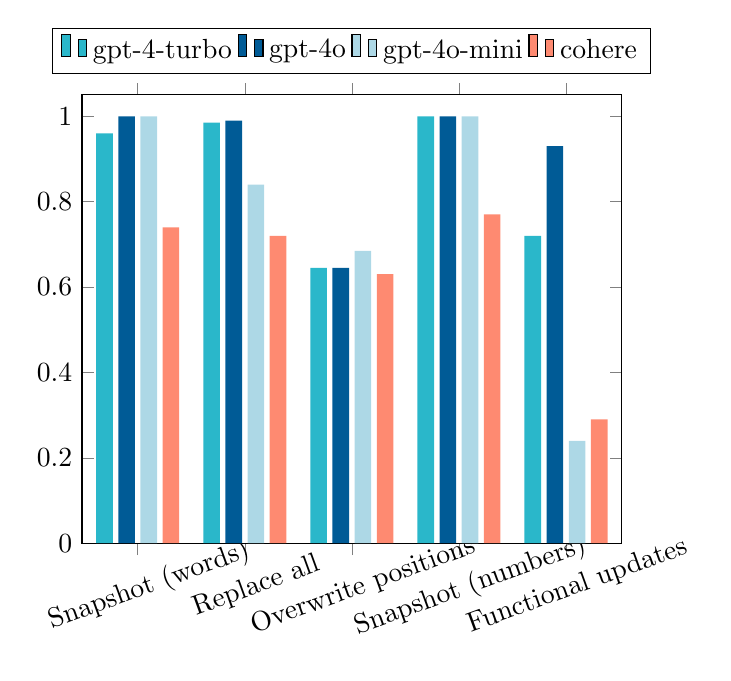
\begin{tikzpicture}
        \begin{axis}[
            ybar,
            bar width=6pt,
            symbolic x coords={Snapshot (words), Replace all, Overwrite positions, Snapshot (numbers), Functional updates},
            xtick=data,
            ymin=0, ymax=1.05,
            legend columns=4,
            legend style={at={(0.5,1.15)}, anchor=north, draw=black},
            enlarge x limits=0.13,
            xticklabel style={rotate=20, anchor=center, yshift=-12pt}
        ]
        
        \addplot[fill={rgb,255:red,42;green,183;blue,202}, draw=none] coordinates {(Snapshot (words),0.96) (Replace all,0.985) (Overwrite positions,0.645) (Snapshot (numbers),1.00) (Functional updates,0.72)};
        \addlegendentry{gpt-4-turbo}
        
        \addplot[fill={rgb,255:red,0;green,91;blue,150}, draw=none] coordinates {(Snapshot (words),1.00) (Replace all,0.99) (Overwrite positions,0.645) (Snapshot (numbers),1.00) (Functional updates,0.93)};
        \addlegendentry{gpt-4o}
        
        \addplot[fill={rgb,255:red,173;green,216;blue,230}, draw=none] coordinates {(Snapshot (words),1.00) (Replace all,0.84) (Overwrite positions,0.685) (Snapshot (numbers),1.00) (Functional updates,0.24)};
        \addlegendentry{gpt-4o-mini}
        
        \addplot[fill={rgb,255:red,254;green,138;blue,113}, draw=none] coordinates {(Snapshot (words),0.74) (Replace all,0.72) (Overwrite positions,0.63) (Snapshot (numbers),0.77) (Functional updates,0.29)};
        \addlegendentry{cohere}
        
        \end{axis}
\end{tikzpicture}}
    \end{subfigure}
    \begin{subfigure}{0.49\columnwidth}
        \resizebox{\textwidth}{!}{    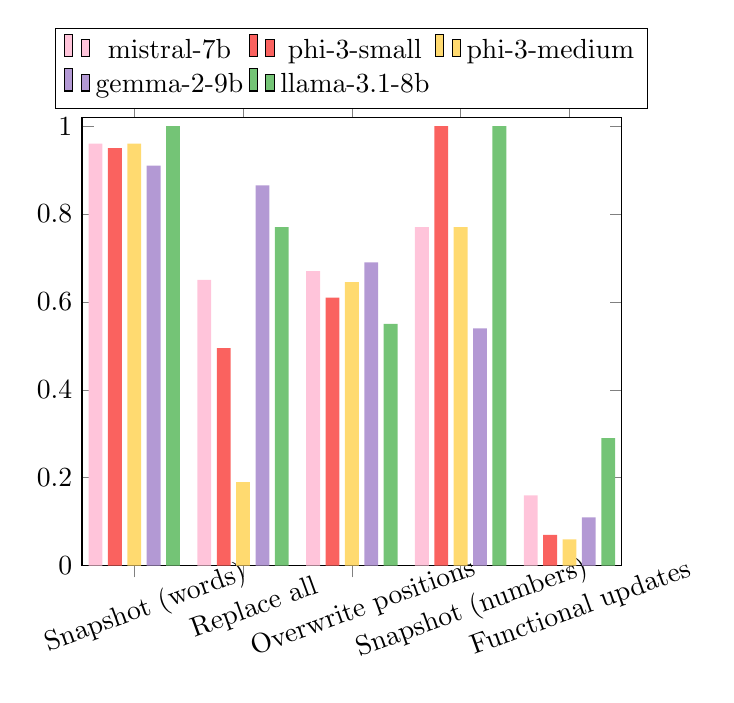
\begin{tikzpicture}
        \begin{axis}[
            ybar,
            bar width=5pt,
            symbolic x coords={Snapshot (words), Replace all, Overwrite positions, Snapshot (numbers), Functional updates},
            xtick=data,
            ymin=0, ymax=1.02,
            legend columns=3,
            legend style={at={(0.5,1.20)}, anchor=north, draw=black},
            enlarge x limits=0.12,
            xticklabel style={rotate=20, anchor=center, yshift=-12pt}
        ]
        
        \addplot[fill={rgb,255:red,255;green,196;blue,218}, draw=none] coordinates {(Snapshot (words),0.96) (Replace all,0.65) (Overwrite positions,0.67) (Snapshot (numbers),0.77) (Functional updates,0.16)};
        \addlegendentry{mistral-7b}
        
        \addplot[fill={rgb,255:red,250;green,98;blue,95}, draw=none] coordinates {(Snapshot (words),0.95) (Replace all,0.495) (Overwrite positions,0.61) (Snapshot (numbers),1.00) (Functional updates,0.07)};
        \addlegendentry{phi-3-small}
        
        \addplot[fill={rgb,255:red,255;green,218;blue,112}, draw=none] coordinates {(Snapshot (words),0.96) (Replace all,0.19) (Overwrite positions,0.645) (Snapshot (numbers),0.77) (Functional updates,0.06)};
        \addlegendentry{phi-3-medium}
        
        \addplot[fill={rgb,255:red,179;green,153;blue,212}, draw=none] coordinates {(Snapshot (words),0.91) (Replace all,0.865) (Overwrite positions,0.69) (Snapshot (numbers),0.54) (Functional updates,0.11)};
        \addlegendentry{gemma-2-9b}
        
        \addplot[fill={rgb,255:red,116;green,196;blue,118}, draw=none] coordinates {(Snapshot (words),1.00) (Replace all,0.77) (Overwrite positions,0.55) (Snapshot (numbers),1.00) (Functional updates,0.29)};
        \addlegendentry{llama-3.1-8b}
        
        \end{axis}
\end{tikzpicture}}
    \end{subfigure}
    \caption{Results for the \textbf{Recall and Edit} tasks.}
    \label{fig:recall}
\end{figure}

\paragraph{Recall and Edit} 
\begin{table}[!h]
    \centering
        \resizebox{0.8\columnwidth}{!}{%
    \begin{tabular}{lllll}
    \toprule
        \textbf{Model} & \textbf{String Search (word)} & \textbf{Snapshot} \\ \hline
gpt-4-turbo    & 1.00 \textcolor{green}{(0.06)} & 1.00 \textcolor{green}{(0.04)} \\ 
gpt-4o         & 1.00 (0.00)                   & 1.00 (0.00)                   \\ 
gpt-4o-mini    & 0.94 \textcolor{red}{(-0.04)}  & 1.00 (0.00)                   \\ 
cohere         & 1.00 (0.00)                   & 1.00 \textcolor{green}{(0.26)} \\ 
mistral-7b     & 1.00 \textcolor{green}{(0.22)} & 0.96 (0.00)                   \\ 
phi-3-small    & 1.00 \textcolor{green}{(0.06)} & 0.99 \textcolor{green}{(0.04)} \\ 
phi-3-medium   & 0.98 \textcolor{red}{(-0.02)}  & 0.87 \textcolor{red}{(-0.09)}  \\ 
gemma-2-9b     & 0.96 \textcolor{red}{(-0.04)}  & 0.96 \textcolor{green}{(0.05)} \\ 
llama-3.1-8b   & 0.98 \textcolor{red}{(-0.02)}  & 1.00 (0.00)                   \\
\bottomrule
    \end{tabular}
    }
    \caption{Ablation study with gibberish context.}
    \label{tab:ablation_gibberish}
\end{table}

Figure \ref{fig:recall} presents the results for the \textbf{Recall and Edit} tasks. While models performed well on basic recall (\textit{Snapshot}), their performance dropped sharply when tasked with making regular edits. A closer analysis of the generated outputs reveals that models struggled with maintaining coherence during edits, often getting trapped in repetitive word loops. For the \textit{Functional Update} task, we deliberately selected simple numerical updates, such as ``Subtract 1 from every number," to ensure the edits were within the models' capabilities. Nevertheless, when comparing performance on \textit{Snapshot (with numbers)} to \textit{Functional Updates}, all models exhibited a steep decline, especially for smaller ones. Analysis of generated outputs revealed that these models frequently deviated from instructions over longer sequences, suggesting difficulties in maintaining consistent rule applications over extended contexts.

Additionally, we conducted a separate ablation study on \textit{Snapshot} and \textit{String Search}. In this study, we replaced meaningful words in the context with gibberish tokens consisting of randomly generated alphabetical characters. As shown in Table \ref{tab:ablation_gibberish}, performance remained largely unchanged, suggesting that semantic meaning was not a significant distractor in these tasks.

\section{Backup: compare with previous works}

\paragraph{Comparison with Theorem 1 of \cite{srikant2024rates}.} While the framework of our proof of Theorem \ref{thm:Srikant-generalize} is mainly inspired by the proof of Theorem 1 of \cite{srikant2024rates}, there are some noteworthy differences. Most importantly, we observe that in the equation beginning from the bottom of Page 7 and continuing to the start of Page 8, the right-most side contains a term
\begin{align}\label{eq:Srikant-error}
-\frac{1}{n-k+1} \mathsf{Tr}\left(\bm{\Sigma}_{\infty}^{-\frac{1}{2}}(\bm{\Sigma}_k - \bm{\Sigma}_{\infty})\bm{\Sigma}_{\infty}^{-\frac{1}{2}}\mathbb{E}[\nabla^2 f(\tilde{\bm{Z}}_k)]\right);
\end{align}
the author argued that ``by taking an expectation to remove conditioning, and defining $\bm{A}_k$ to be $\mathbb{E}[\nabla^2 f(\tilde{\bm{Z}}_k)]$'', this term can be transformed to the term
\begin{align}\label{eq:Srikant-wrong}
-\frac{1}{n-k+1} \mathsf{Tr}\left(\bm{A}_k \left(\bm{\Sigma}_{\infty}^{-\frac{1}{2}} \mathbb{E}[\bm{\Sigma}_k]\bm{\Sigma}_{\infty}^{-\frac{1}{2}}-\bm{I}\right)\right)
\end{align}
in the expression of Theorem 1. However, we note that the function $f(\cdot)$, as defined on Page 6 as the solution to the Stein's equation with respect to $\tilde{h}(\cdot)$, is \emph{dependent on} $\mathcal{F}_{k-1}$; in fact, $f$ corresponds to the function $f_k$ in our proof. Consequently, the terms $\bm{A}_k = \mathbb{E}[\nabla^2 f(\tilde{\bm{Z}}_k)]$ (which is actually a conditional expectation with respect to $\mathcal{F}_{k-1}$), and $\bm{\Sigma}_k$ (which corresponds to $\bm{V}_k$ in our proof), are confounded by $\mathcal{F}_{k-1}$ and hence \emph{not independent}. Therefore, taking expectation, with respect to $\mathcal{F}_0$, on \eqref{eq:Srikant-error} should yield
\begin{align}\label{eq:Srikant-right}
-\frac{1}{n-k+1} \mathbb{E}\left\{\mathsf{Tr}\left(\bm{A}_k \left(\bm{\Sigma}_{\infty}^{-\frac{1}{2}} \bm{\Sigma}_k\bm{\Sigma}_{\infty}^{-\frac{1}{2}}-\bm{I}\right)\right)\right\}
\end{align}
Notice that the expectation is taken over the trace as a whole, instead of only $\bm{\Sigma}_k$. However, also due to the confounding bewteen $\bm{A}_k$ and $\bm{\Sigma}_k$, there is no guarantee that the sum of \eqref{eq:Srikant-right} is bounded as shown in the proof of Theorem 2 in \cite{srikant2024rates} on page 10. In other words, the framework of the proof needs a substantial correction to obtain a meaningful Berry-Esseen bound. 

Our solution in the proof of Theorem \ref{thm:Srikant-generalize} is to replace the matrix $\bm{Q}=\sqrt{n-k+1}\bm{\Sigma}_{\infty}$, as defined on Page 6 of \cite{srikant2024rates}, with the matrix $\bm{P}_k$, following the precedent of \cite{JMLR2019CLT}. This essentially eliminates the term \eqref{eq:Srikant-right}, but would require $\bm{P}_k$ to be measurable with respect to $\mathcal{F}_{k-1}$. For this purpose, we impose the assumption that $\bm{P}_1 = n\bm{\Sigma}_n$ almost surely, also following the precedent of \cite{JMLR2019CLT}. The relaxation of this assumption would be addressed in Theorem \ref{thm:Berry-Esseen-mtg}. 

Another important improvement we made in Theroem \ref{thm:Srikant-generalize} is to tighten the upper bound through a closer scrutiny of the smoothness of the solution to the Stein's equation, as is indicated in Proposition \ref{prop:Stein-smooth}. This paves the way for Corollary \ref{cor:Wu}, the proof of which we present in the next subsection. 


\begin{table}[!htbp] \centering
  \caption{Human Choices and Predictions About GenAI Choice in the Same Problem: Heterogeneity by Exposure and Attitudes (Pooled)}
\begin{adjustbox}{scale=0.8}
\begin{tabular}{@{\extracolsep{5pt}}lccccc}
% \\[-1.8ex]\hline
% \hline \\[-1.8ex]
\toprule
& \multicolumn{5}{c}{\textit{Dependent variable: Prediction}} \
\cr \cline{2-6}
\\[-1.8ex] & \multicolumn{1}{c}{Heavy User} & \multicolumn{1}{c}{Text-Based LLM User} & \multicolumn{1}{c}{Paid User} & \multicolumn{1}{c}{Agree AI Similar} & \multicolumn{1}{c}{Agree AI Better}  \\
\\[-1.8ex] & (1) & (2) & (3) & (4) & (5) \\
% \hline \\[-1.8ex]
\midrule
 X$\times$Heavy User & -0.056$^{}$ & & & & \\
& (0.052) & & & & \\
 X$\times$Text-Based LLM User & & 0.082$^{**}$ & & & \\
& & (0.040) & & & \\
 X$\times$Paid User & & & -0.001$^{}$ & & \\
& & & (0.072) & & \\
 X$\times$Agree AI Similar & & & & 0.033$^{}$ & \\
& & & & (0.045) & \\
 X$\times$Agree AI Better & & & & & 0.019$^{}$ \\
& & & & & (0.017) \\
 Problem FE & Yes & Yes & Yes & Yes & Yes \\
 X$\times$Problem FE & Yes & Yes & Yes & Yes & Yes \\
 G$\times$Problem FE & Yes & Yes & Yes & Yes & Yes \\
% \hline \\[-1.8ex]
\midrule
 Observations & 2700 & 2700 & 2700 & 2700 & 2700 \\
 % Residual Std. Error & 22.874 & 22.851 & 22.863 & 22.847 & 22.895 \\
% \hline
% \hline \\[-1.8ex]
\bottomrule
\textit{Note:} & \multicolumn{5}{r}{Standard errors are clustered at the problem level. $^{*}$p$<$0.1; $^{**}$p$<$0.05; $^{***}$p$<$0.01} \\
% \multicolumn{6}{r}\textit{} \\
\end{tabular}
\end{adjustbox}
\label{tab:group} \end{table}


\paragraph{Match and Compare}
 As shown in Figure \ref{fig:match}, model performance in the \textbf{Match and Compare} tasks was relatively consistent across different model sizes. Given that counting is a well-known weakness in LLMs, it is unsurprising that all models struggled significantly with the counting task, though GPT models performed slightly better than others. However, models generally succeeded in identifying the duplicates (in \textit{Find duplicates}), and primarily struggled with the counting aspect -- which requires tracking and updating an integer state, a skill that is more similar to stateful processing. This suggests that relying solely on counting-based tests \cite{song2024countingstars} could overly bias the evaluation and fail to capture broader model capabilities. The results also indicate that models exhibit some ability to recognize relative positions and group associations, but their accuracy remains limited (ranging between 0.6-0.8). A closer examination of model generations reveals an overwhelming tendency for the models to produce false positive errors -- models often answer “yes” when the correct answer is “no”, while making very few false negative errors. This means that when the relationship is correct, the models can more reliably identify it. This may stem from a combination of their inherent inclination to agree and the difficulty in recognizing relative comparisons and associations.

% \begin{figure}[h]
%     \centering
%     \includegraphics[width=0.92\columnwidth]{images/difference.png}
%     \caption{Results for \textbf{Spot the Differences }tasks.}
%     \label{fig:difference}
% \end{figure}

\begin{figure}[h]
\centering
\resizebox{0.9\columnwidth}{!}{
 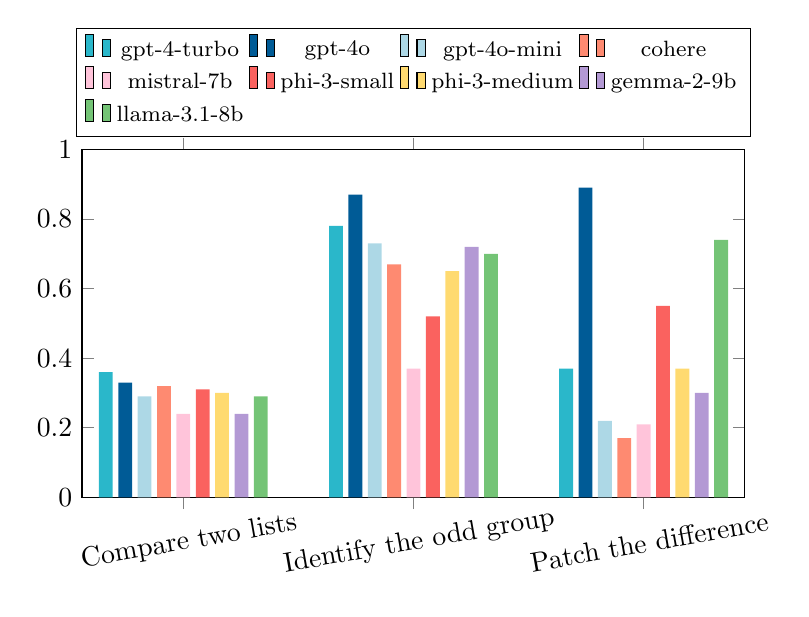
\begin{tikzpicture}
        \begin{axis}[
            ybar,
            bar width=5pt,
            symbolic x coords={Compare two lists, Identify the odd group, Patch the difference},
            xtick=data,
            ymin=0, ymax=1.0,
            legend columns=4,
            legend style={at={(0.5,1.35)}, anchor=north, draw=black, font=\footnotesize},
            enlarge x limits=0.22,
            xticklabel style={rotate=10, anchor=center, yshift=-12pt},
            width=10cm, height=6cm,
        ]
        
        \addplot[fill={rgb,255:red,42;green,183;blue,202}, draw=none] coordinates {(Compare two lists,0.36) (Identify the odd group,0.78) (Patch the difference,0.37)};
        \addlegendentry{gpt-4-turbo}
        
        \addplot[fill={rgb,255:red,0;green,91;blue,150}, draw=none] coordinates {(Compare two lists,0.33) (Identify the odd group,0.87) (Patch the difference,0.89)};
        \addlegendentry{gpt-4o}
        
        \addplot[fill={rgb,255:red,173;green,216;blue,230}, draw=none] coordinates {(Compare two lists,0.29) (Identify the odd group,0.73) (Patch the difference,0.22)};
        \addlegendentry{gpt-4o-mini}
        
        \addplot[fill={rgb,255:red,254;green,138;blue,113}, draw=none] coordinates {(Compare two lists,0.32) (Identify the odd group,0.67) (Patch the difference,0.17)};
        \addlegendentry{cohere}
        
        \addplot[fill={rgb,255:red,255;green,196;blue,218}, draw=none] coordinates {(Compare two lists,0.24) (Identify the odd group,0.37) (Patch the difference,0.21)};
        \addlegendentry{mistral-7b}
        
        \addplot[fill={rgb,255:red,250;green,98;blue,95}, draw=none] coordinates {(Compare two lists,0.31) (Identify the odd group,0.52) (Patch the difference,0.55)};
        \addlegendentry{phi-3-small}
        
        \addplot[fill={rgb,255:red,255;green,218;blue,112}, draw=none] coordinates {(Compare two lists,0.30) (Identify the odd group,0.65) (Patch the difference,0.37)};
        \addlegendentry{phi-3-medium}
        
        \addplot[fill={rgb,255:red,179;green,153;blue,212}, draw=none] coordinates {(Compare two lists,0.24) (Identify the odd group,0.72) (Patch the difference,0.30)};
        \addlegendentry{gemma-2-9b}
        
        \addplot[fill={rgb,255:red,116;green,196;blue,118}, draw=none] coordinates {(Compare two lists,0.29) (Identify the odd group,0.70) (Patch the difference,0.74)};
        \addlegendentry{llama-3.1-8b}
        
        \end{axis}
    \end{tikzpicture}}
    \caption{Results for \textbf{Spot the Differences }tasks.}
    \label{fig:difference}
\end{figure}

\paragraph{Spot the Differences}
As shown in Figure \ref{fig:difference}, performance across all models are poor on \textit{Compare Two Lists}, suggesting inherent difficulties in cross-referencing information across long contexts, even for larger models.  GPT-4o and the LLaMA model significantly outperform the others in the \textit{Identify the Odd Group} task, highlighting a general weakness in detecting contextual differences by the other models. However, an 8B LLaMA model outperforms both equivalently-sized models and even GPT-4 in this task, suggesting that model size alone was not the determining factor. This indicates that architectural differences, training objectives, or specific inductive biases may contribute to improved performance in comparative memory utilization.


\paragraph{Compute on Sets and Lists}
The tasks in this category require models to recognize and process group structures within the context, and performance gradually declines as the complexity of the task increases (see Table \ref{tab:lists}). For instance, in comparing the \textit{Group Membership} task with the \textit{String Search} task, where the former requires identifying which list a word belongs to rather than simply determining its presence, the performance of open-source models drops considerably. Similarly, in comparing the \textit{Group Association} task with the \textit{Group Membership} task, where the former requires determining whether two words belong to the same group, all models exhibit a noticeable decline in performance. The decline becomes even more pronounced when comparing the \textit{ Group Association (alternating)} variant of the task to the standard \textit{Group Association} task. Here, the context involves alternating repeated groups rather than simple group structures, which further challenges the models' abilities to handle partitioned contexts effectively.

An interesting observation was found during the \textit{Iterate} task. In an ablation study, we modified the task to require returning the first words in each list instead of the last words (making it more similar to the \textit{Batch Search} task). The performance sharply declines when models are asked to return the last words, despite their strong information-fetching capabilities. This suggests that, while the models can retrieve information effectively, they struggle to accurately recognize and process partitions within the context.


\begin{table}[h!]
\large
\centering
\begin{adjustbox}{width=\columnwidth} % Automatically fit within column width
\begin{tabular}{|c|p{0.75\columnwidth}|} % Adjust the second column width proportionally
\hline
\textbf{Symbol} & \textbf{Explanation} \\ \hline
$q^{\text{obj}} \in SE(2)$ & Object pose \\ \hline
$q^{\text{robot}} \in \mathbb{R}^9$ & Robot configuration (9 DoF robot joint position) \\ \hline
$q^{\text{obj}}_\text{sg} \in SE(2)$ & Subgoal object pose \\ \hline
$q^{\text{robot}}_\text{sg} \in SE(3) \times \mathbb{R}^3$ & Subgoal robot configuration (End-effector pose in $SE(3)$ and gripper tip positions in 3D space) \\ \hline
$q^{\text{obj}}_{\text{init}} \in SE(2)$ & Initial object pose of the task \\ \hline
$q^{\text{robot}}_{\text{init}} \in \mathbb{R}^9$ & Initial robot configuration of the task (9 DoF robot joint position) \\ \hline
$q^{\text{obj}}_{\text{goal}} \in SE(2)$ & Goal object pose of the task \\ \hline
$s$ & State \\ \hline
% $sg$ & Subgoal information (e.g., subgoal object pose, robot configuration) \\ \hline
\end{tabular}
\end{adjustbox}
\caption{Notation table for task parameters}
\label{tab:state_notation}
\end{table}

\paragraph{Stateful Processing}

\begin{figure}[t!]
    \centering
    \begin{subfigure}{0.49\columnwidth}
        \resizebox{\textwidth}{!}{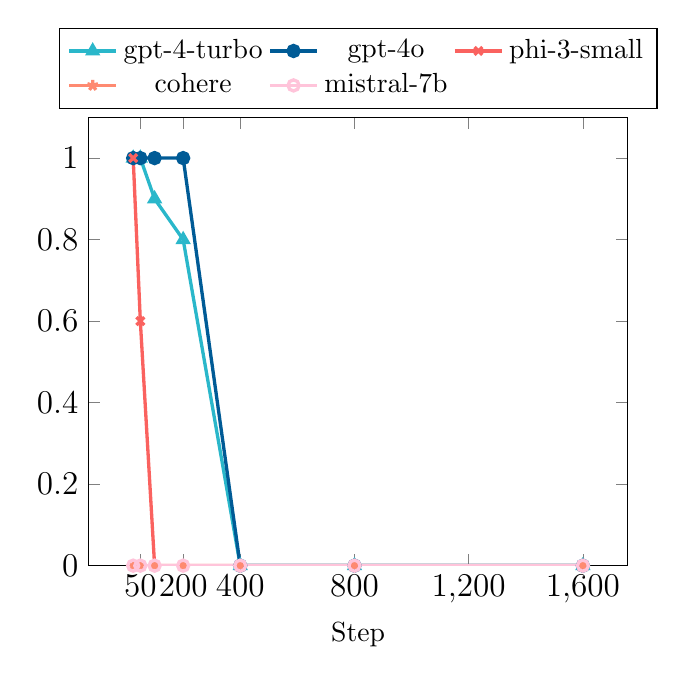
\begin{tikzpicture}
    \begin{axis}[
        xlabel={Step},
        legend style={at={(0.5,1.2)}, anchor=north, cells={align=left}, legend columns=3},
        ymin=0, ymax=1.1,
        xtick={50, 200, 400, 800, 1200, 1600},
        ytick={0,0.2,0.4,0.6,0.8,1.0},
        grid=none,
        tick label style={font=\large}
    ]

    % GPT-4-Turbo
    \addplot[mark=triangle, very thick, color={rgb,255:red,42;green,183;blue,202}] coordinates {
        (25,1.0) (50,1.0) (100,0.9) (200,0.8) (400,0.0) (800,0.0) (1600,0.0)
    };
    \addlegendentry{gpt-4-turbo}

    % GPT-4o
    \addplot[mark=*, very thick, color={rgb,255:red,0;green,91;blue,150}] coordinates {
        (25,1.0) (50,1.0) (100,1.0) (200,1.0) (400,0.0) (800,0.0) (1600,0.0)
    };
    \addlegendentry{gpt-4o}



    % Phi-3-Small
    \addplot[mark=x, very thick, color={rgb,255:red,250;green,98;blue,95}] coordinates {
        (25,1.0) (50,0.6) (100,0.0) (200,0.0) (400,0.0) (800,0.0) (1600,0.0)
    };
    \addlegendentry{phi-3-small}

    % Cohere
    \addplot[mark=star, very thick, color={rgb,255:red,254;green,138;blue,113}] coordinates {
        (25,0.0) (50,0.0) (100,0.0) (200,0.0) (400,0.0) (800,0.0) (1600,0.0)
    };
    \addlegendentry{cohere}

    % Mistral-7B
    \addplot[mark=o, very thick, color={rgb,255:red,255;green,196;blue,218}] coordinates {
        (25,0.0) (50,0.0) (100,0.0) (200,0.0) (400,0.0) (800,0.0) (1600,0.0)
    };
    \addlegendentry{mistral-7b}
    
    \end{axis}
\end{tikzpicture}}
    \end{subfigure}
    \begin{subfigure}{0.49\columnwidth}
        \resizebox{\textwidth}{!}{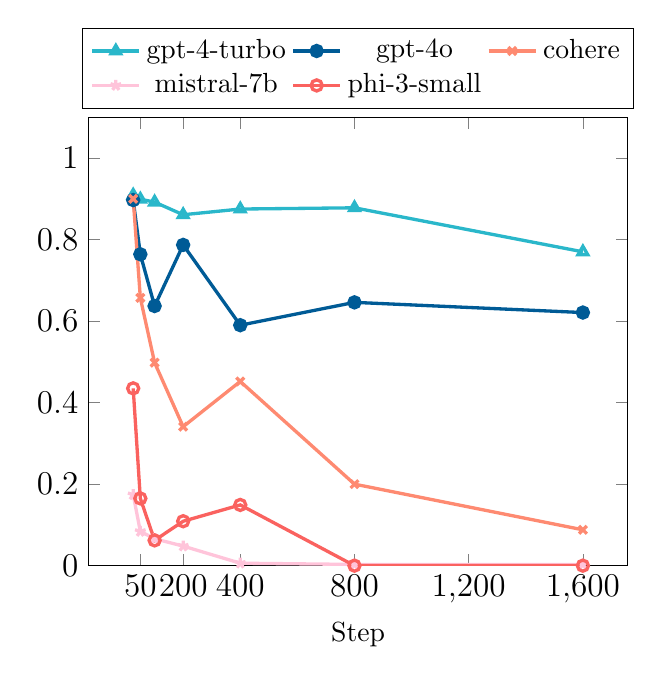
\begin{tikzpicture}
    \begin{axis}[
        xlabel={Step},
        legend style={at={(0.5,1.2)}, anchor=north, cells={align=left}, legend columns=3},
        ymin=0, ymax=1.1,
        xtick={50, 200, 400, 800, 1200, 1600},
        ytick={0,0.2,0.4,0.6,0.8,1.0},
        grid=none,
        tick label style={font=\large}
    ]

    % GPT-4-Turbo
    \addplot[mark=triangle, very thick, color={rgb,255:red,42;green,183;blue,202}] coordinates {
        (25,0.909) (50,0.899) (100,0.892) (200,0.861) (400,0.875) (800,0.878) (1600,0.770)
    };
    \addlegendentry{gpt-4-turbo}

    % GPT-4o
    \addplot[mark=*, very thick, color={rgb,255:red,0;green,91;blue,150}] coordinates {
        (25,0.897) (50,0.764) (100,0.637) (200,0.787) (400,0.590) (800,0.646) (1600,0.621)
    };
    \addlegendentry{gpt-4o}

    % Cohere
    \addplot[mark=x, very thick, color={rgb,255:red,254;green,138;blue,113}] coordinates {
        (25,0.900) (50,0.657) (100,0.498) (200,0.341) (400,0.452) (800,0.200) (1600,0.088)
    };
    \addlegendentry{cohere}

    % Mistral-7B
    \addplot[mark=star, very thick, color={rgb,255:red,255;green,196;blue,218}] coordinates {
        (25,0.174) (50,0.084) (100,0.066) (200,0.048) (400,0.006) (800,0.003) (1600,0.003)
    };
    \addlegendentry{mistral-7b}

    % Phi-3-Small
    \addplot[mark=o, very thick, color={rgb,255:red,250;green,98;blue,95}] coordinates {
        (25,0.435) (50,0.165) (100,0.062) (200,0.109) (400,0.149) (800,0.000) (1600,0.000)
    };
    \addlegendentry{phi-3-small}
    
    \end{axis}
\end{tikzpicture}}
    \end{subfigure}
    \caption{Ablation study on the number of operation steps for the \textbf{quantity state} (left) and\textbf{ set state }(right).}
    \label{fig:ablation_state_step}
\end{figure}



Table \ref{tab:state} presents the results for the \textbf{Stateful Processing} tasks, where performance gaps among models are the most pronounced. The GPT-4(o) models perform well on integer state tracking, while most other models struggle (near zero accuracy). For set state tracking, larger models generally perform better.

We conducted an ablation study to examine how the number of operation steps influences performance of five selected models (Fig. \ref{fig:ablation_state_step}). For quantity state tracking, GPT-4(o) models perform well within fewer than 200 steps but experience a sharp decline in accuracy beyond this threshold. For set state tracking, the performance decline is more gradual. The differences in performance drop between the two tasks can be attributed to the nature of the two tasks. While tracking an integer state might seem simpler than tracking a set, it actually requires the model to maintain and apply every operation sequentially to compute the final value. In contrast, for set state, the fixed size of the set makes more recent operations more relevant to the final state, reducing the need for exhaustive step-by-step tracking. Nevertheless, even in this scenario, all models show a clear inability to handle longer or more complex operation sequences effectively. Interestingly, GPT-4 model outperformed GPT-4o at this task, suggesting potential optimization trade-offs may have affected its ability to manage set-based updates. 

Overall, while larger models like GPT-4(o) exhibit some ability to track state over time, their effectiveness rapidly deteriorates as task complexity increases. Smaller models, in particular, struggle to track operations over time, pointing to significant gaps in their ability to manage and process sequential dependencies critical for state tracking tasks.

\subsection{Results on Composite Tests}

\section{Simple Construction of Projective Compositions}
\label{sec:comp_coord}

It is not clear apriori that projective compositional distributions satisfying Definition \ref{def:proj_comp} ever exist, much less that there is any straightforward way to sample from them.
To explore this, we first restrict attention to perhaps the simplest setting, where the projection functions $\{\Pi_i\}$ are
just coordinate restrictions.
This setting is meant to generalize the intuition we had
in the CLEVR example of Figure~\ref{fig:len_gen},
where different objects were composed in disjoint regions of the image.
We first define the construction of the composed distribution,
and then establish its theoretical properties.








\subsection{Defining the Construction}
Formally, suppose we have a set of distributions
$(p_1, p_2, \ldots, p_k)$ that we wish to compose;
in our running CLEVR example, each $p_i$ is the distribution of images
with a single object at position $i$.
Suppose also we have some reference distribution $p_b$,
which can be arbitrary, but should be thought of as a 
``common background'' to the $p_i$s.
Then, one popular way to construct a composed distribution
is via the \emph{compositional operator} defined below.
(A special case of this construction is used in \citet{du2023reduce}, for example).


\begin{definition}[Composition Operator]
    \label{def:comp_oper}
    Define the \emph{composition operator} $\cC$ acting on an arbitrary set of distributions $(p_b, p_1, p_2, \ldots)$ by
    \begin{align}
    \label{eq:comp_oper}
    \cC[\vec{p}] := \cC[p_b, p_1, p_2, \dots](x) := \frac{1}{Z} p_b(x) \prod_i \frac{p_i(x)}{p_b(x)},
    \end{align}
    where $Z$ is the appropriate normalization constant. We name $\cC[\vec{p}]$ the \emph{composed distribution}, and the score of $\cC[\vec{p}]$ the \emph{compositional score}:
    \begin{align}
    \label{eqn:comp_score}
    &\grad_x \log \cC[\vec{p}](x)  \\
    &= \grad_x \log p_b(x) + \sum_i \left( \grad_x \log p_i(x) - \grad_x \log p_b(x) \right). \notag
    \end{align}
\end{definition}
Notice that if $p_b$ is taken to be the unconditional distribution then this is exactly the Bayes-composition.


\vspace{-0.5em}
\subsection{When does the Composition Operator Work?}
We can always apply the composition operator to any set of distributions,
but when does this actually yield a ``correct'' composition
(according to Definition~\ref{def:proj_comp})?
One special case is when each distribution $p_i$ is
``active'' on a different, non-overlapping set of coordinates.
We formalize this property below
as \emph{Factorized Conditionals} (Definition~\ref{def:factorized}).
The idea is, 
each distribution $p_i$
must have a particular set of ``mask'' coordinates $M_i \subseteq [n]$ which it
samples in a characteristic way,
while independently sampling all other coordinates
from a common background distribution.
If a set of distributions $(p_b, p_1, p_2, \ldots)$ has this
\emph{Factorized Conditional} structure, then 
the composition
operator will produce a projective composition (as we will prove below).



\begin{definition}[Factorized-Conditionals]
\label{def:factorized}

We say a set of distributions $(p_b, p_1, p_2, \dots p_k)$
over $\R^n$
are \emph{Factorized Conditionals} if
there exists a partition of coordinates $[n]$
into disjoint subsets $M_b, M_1, \dots M_k$ such that:
\begin{enumerate}
    \setlength{\itemsep}{1pt}
    \item $(x|_{M_i}, x|_{M_i^c})$ are independent under $p_i$.
    \item $(x|_{M_b}, x|_{M_1}, x|_{M_2}, \dots, x|_{M_k})$
    are mutually independent under $p_b$.
    \item $p_i(x|_{M_i^c}) = p_b(x|_{M_i^c})$.
\end{enumerate}

Equivalently, if we have:
\begin{align}
    p_i(x) &= p_i(x|_{M_i}) p_b(x|_{M_i^c}), \text{ and} \label{eqn:cc-cond}\\
    p_b(x) &= p_b(x|_{M_b}) \prod_{i \in [k]} p_b(x|_{M_i}). \notag
\end{align}
\end{definition}
\vspace{-1em}
Equation~\eqref{eqn:cc-cond} means that each $p_i$
can be sampled by first sampling $x \sim p_b$,
and then overwriting the coordinates of $M_i$
according to some other distribution (which can be specific to distribution $i$).
For instance, the experiment of Figure~\ref{fig:len_gen}
intuitively satisfies this property, since 
each of the conditional distributions could essentially be sampled
by first sampling an empty background image ($p_b$), then ``pasting''
a random object in the appropriate location (corresponding to pixels $M_i$).
If a set of distributions obey this Factorized Conditional structure,
then we can prove that the composition operator $\cC$
yields a correct projective composition,
and reverse-diffusion correctly samples from it.
Below, let $N_t$ denote the noise operator of the
diffusion process\footnote{Our results are agnostic to the specific diffusion noise-schedule and scaling used.} at time $t$.

\begin{theorem}[Correctness of Composition]
\label{lem:compose}
Suppose a set of distributions $(p_b, p_1, p_2, \dots p_k)$
satisfy Definition~\ref{def:factorized},
with corresponding masks $\{M_i\}_i$.
Consider running the reverse-diffusion SDE 
using the following compositional scores at each time $t$:
\begin{align}
s_t(x_t) &:= \grad_x \log \cC[p_b^t, p_1^t, p_2^t, \ldots](x_t),
\end{align}
where $p_i^t := N_t[p_i]$ are the noisy distributions.
Then, the distribution of the generated sample $x_0$ at time $t=0$ is:
\begin{align}
\label{eqn:p_hat}
\hat{p}(x) := p_b(x|_{M_b}) \prod_i p_i(x|_{M_i}).
\end{align}
In particular,
$\hat{p}(x|_{M_i}) = p_i(x|_{M_i})$ for all $i$,
and so
$\hat{p}$ is a projective composition
with respect to projections $\{\Pi_i(x) := x|_{M_i}\}_i$,
per Definition \ref{def:proj_comp}.
\end{theorem}




Unpacking this, Line \ref{eqn:p_hat} says that the final generated distribution
$\hat{p}(x)$ can be sampled by
first sampling
the coordinates $M_b$ according to $p_b$ (marginally),
then independently sampling 
coordinates $M_i$ according to $p_i$ (marginally) for each $i$.
Similarly, by assumption, $p_i(x)$ can be sampled by first sampling the coordinates $M_i$ in some specific way, and then independently sampling the remaining coordinates according to $p_b$. Therefore Theorem \ref{lem:compose} says that $\hat{p}(x)$ samples the coordinates \emph{$M_i$ exactly as they would be sampled by $p_i$}, for each $i$ we wish to compose. 

\begin{proof}(Sketch) \small
Since $\vec{p}$ satisfies Definition \ref{def:factorized}, we have
\begin{align*}
&\cC[\vec{p}](x) := p_b(x) \prod_i \frac{p_i(x)}{p_b(x)} \notag 
= p_b(x) \prod_i \frac{p_b(x_t|_{M_i^c}) p_i(x|_{M_i})}{p_b(x|_{M_i^c})p_b(x|_{M_i})} \notag \\
&= p_b(x) \prod_i \frac{p_i(x|_{M_i})}{p_b(x|_{M_i})} \notag 
= p_b(x|_{M_b}) \prod_i p_i(x_t|_{M_i}) := \hat{p}(x).
\end{align*}
The sampling guarantee follows from the commutativity of composition with the diffusion noising process, i.e. $\cC[\vec{p^t}]= N_t[\cC[\vec{p}]]$. 
The complete proof is in Appendix \ref{app:compose_pf}.
\end{proof}

\begin{remark}
In fact, Theorem~\ref{lem:compose} still holds under any orthogonal transformation of the variables,
because the diffusion noise process commutes with orthogonal transforms.
We formalize this as Lemma~\ref{lem:orthogonal_sampling}.
\end{remark}

\begin{remark}
Compositionality is often thought of in terms of orthogonality between scores.
Definition \ref{def:factorized} implies orthogonality between the score differences that appear in the composed score \eqref{eqn:comp_score}:
$\grad_x \log p_i^t(x_t) - \grad_x \log p_b^t(x_t),$
but the former condition is strictly stronger
(c.f. Appendix \ref{app:score_orthog}).
\end{remark}

\begin{remark}
Notice that the composition operator $\cC$
can be applied to a set of Factorized Conditional
distributions
without knowing the coordinate partition $\{M_i\}$.
That is, we can compose distributions and compute scores
without knowing apriori exactly ``how'' these distributions are supposed to compose
(i.e. which coordinates $p_i$ is active on).
This is already somewhat remarkable, and we will see a much
stronger version of this property in the next section.
\end{remark}

\textbf{Importance of background.}
Our derivations highlight the crucial role of the background
distribution $p_b$ for the composition operator  
(Definition~\ref{def:comp_oper}).
While prior works have taken $p_b$ to be an unconditional distribution and the $p_i$'s its associated conditionals,
our results suggest this is not always the optimal choice -- in particular,
it may not satisfy a Factorized Conditional structure (Definition~\ref{def:factorized}). Figure~\ref{fig:len_gen_monster} demonstrates this empirically: settings (a) and (b) attempt to compose the same distributions using different backgrounds -- empty (a) or unconditional (b) -- with very different results.

\subsection{Approximate Factorized Conditionals in CLEVR.}
\label{sec:clevr-details}

In \cref{fig:len_gen_monster} we explore compositional length-generalization (or lack thereof) in three different setting, two of which (\cref{fig:len_gen_monster}a and \ref{fig:len_gen_monster}c) approximately satisfy \cref{def:factorized}. In this section we explicitly describe how our definition of Factorized Conditionals approximately captures the CLEVR settings of Figures \ref{fig:len_gen_monster}a and \ref{fig:len_gen_monster}c. The setting of \ref{fig:len_gen_monster}b does not satisfy our conditions, as discussed in \cref{sec:problematic-compositions}.

\textbf{Single object distributions with empty background.}
This is the setting of both \cref{fig:len_gen} and \cref{fig:len_gen_monster}a.
The background distribution $p_b$ 
over $n$ pixels is images of an empty scene with no objects.
For each $i \in \{1,\ldots,L\}$ (where $L=4$ in \cref{fig:len_gen} and $L=9$ in \cref{fig:len_gen_monster}a), define the set $M_i \subset [n]$ 
as the set of pixel indices surrounding location $i$.
($M_i$ should be thought of as a ``mask'' that
that masks out objects at location $i$).
Let $M_b := (\cup_i M_i)^c$ be the remaining
pixels in the image.
Then, we claim the distributions $(p_b, p_1, \ldots, p_L)$
form approximately
Factorized Conditionals, with corresponding
coordinate partition $\{M_i\}$.
This is essentially because each distribution $p_i$
matches the background $p_b$ on all pixels except those surrounding
location $i$ (further detail in Appendix~\ref{app:clevr-details}).
Note, however, that the conditions of Definition~\ref{def:factorized}
do not \emph{exactly} hold in the experiment of Figure~\ref{fig:len_gen} -- there is still some dependence between
the masks $M_i$, since objects can cast shadows or even occlude each other.
Empirically, these deviations 
have greater impact
when composing many objects, as seen in \cref{fig:len_gen_monster}a.


\textbf{Bayes composition with cluttered distributions.}
In \cref{fig:len_gen_monster}c we replicate CLEVR experiments in  \citet{du2023reduce, liu2022compositional} where the images contain many objects (1-5) and the conditions label the location of one randomly-chosen object. It turns out the unconditional together with the conditionals can approximately act as Factorized Conditionals in ``cluttered'' settings like this one. The intuition is that if the conditional distributions each contain one specific object plus many independently sampled random objects (``clutter''), then the unconditional distribution \emph{almost} looks like independently sampled random objects, which together with the conditionals \emph{would} satisfy Definition \ref{def:factorized} (further discussion in Appendix \ref{app:clevr-details} and \ref{app:bayes_connect}). This helps to explain the length-generalization observed in \citet{liu2022compositional} and verified in our experiments (\cref{fig:len_gen_monster}c).







\section{Projective Composition in Feature Space}
\label{sec:comp_feature}

\begin{figure}
    \centering
    \includegraphics[width=1.0\linewidth]{figures/feat-space-vis.png}
    \caption{A commutative diagram illustrating Theorem~\ref{lem:transform_comp}.
    Performing composition in pixel space is equivalent 
    to encoding into a feature space ($\cA$),
    composing there,
    and decoding back
    to pixel space ($\cA^{-1}$).
    }
    \label{fig:feat-space-vis}
\end{figure}

So far we have focused on the setting where the projection functions $\Pi_i$ are simply projections onto coordinate subsets $M_i$ in the native space (e.g. pixel space).
This covers simple examples like Figure~\ref{fig:len_gen} but does not include more realistic situations such as Figure~\ref{fig:style-content},
where the properties to be composed are more abstract.
For example a property like ``oil painting'' does not correspond to projection
onto a specific subset of pixels in an image.
However, we may hope that there exists some conceptual feature space
in which ``oil painting'' does correspond to a particular subset of variables.
In this section, we extend our results to the case where the composition occurs in some conceptual feature space, and each distribution to be composed
corresponds to some particular subset of \emph{features}.


Our main result is a featurized analogue of Theorem~\ref{lem:compose}:
if there exists \emph{any} invertible transform $\cA$
mapping into a feature space
where Definition \ref{def:factorized} holds,
then the composition operator (Definition~\ref{def:comp_oper})
yields a projective composition in this feature space, as shown in Figure~\ref{fig:feat-space-vis}.

\begin{theorem}[Feature-space Composition]
\label{lem:transform_comp}
Given distributions $\vec{p} := (p_b, p_1, p_2, \dots p_k)$,
suppose there exists a diffeomorphism $\cA: \R^n \to \R^n$
such that
$(\cA \sharp p_b, \cA \sharp p_1, \dots \cA \sharp p_k)$
satisfy Definition~\ref{def:factorized},
with corresponding partition $M_i \subseteq [n]$.
Then, the composition $\hat{p} := \cC[\vec{p}]$ satisfies:
\begin{align}
\label{eqn:p_hat_A}
\cA \sharp \hat{p}(z)
\equiv
(\cA \sharp p_b (z))|_{M_b} \prod_{i=1}^k (\cA \sharp p_i(z))|_{M_i}.
\end{align}
Therefore, $\hat{p}$
is a projective composition of $\vec{p}$ w.r.t. projection functions
$\{\Pi_i(x) := \cA(x)|_{M_i}\}$.
\end{theorem}
This theorem is remarkable because it means we can
compose distributions $(p_b, p_1, p_2, \dots)$ in the base space,
and this composition will ``work correctly'' in the feature space
automatically (Equation~\ref{eqn:p_hat_A}),
without us ever needing to compute or even know the feature transform $\cA$
explicitly.



Theorem~\ref{lem:transform_comp} may apriori seem too strong
to be true, since it somehow holds for all feature spaces $\cA$
simultaneously.
The key observation underlying Theorem~\ref{lem:transform_comp} 
is that the composition operator $\cC$ behaves
well under reparameterization.
\begin{lemma}[Reparameterization Equivariance]
\label{lem:reparam}
The composition operator of Definition~\ref{def:comp_oper}
is reparameterization-equivariant. That is,
for all diffeomorphisms $\cA: \R^n \to \R^n$
and all tuples of distributions $\vec{p} = (p_b, p_1, p_2, \dots, p_k)$,
\begin{align}
 \cC[ \cA \sharp \vec{p}] =  \cA \sharp \cC[\vec{p}].
\end{align}
\end{lemma}
\arxiv{\footnote{
For example (separate from our goals in this paper):
Classifier-Free-Guidance can be seen as an instance of the composition operator.
Thus, Lemma~\ref{lem:reparam} implies that performing CFG
in latent space is \emph{equivalent} to CFG in pixel-space,
assuming accurate score-models in both cases.}}
\arxiv{This lemma is potentially of independent interest:
reparametrization-equivariance
is a very strong property which is typically not satisfied by
standard operations between probability distributions---
for example, the ``simple product'' $p_1(x)p_2(x)$ does not satisfy it---
so it is mathematically notable that the composition operator 
has this structure.
Lemma~\ref{lem:reparam} and Theorem~\ref{lem:transform_comp}
are proved in Appendix \ref{app:param-indep}.}

This lemma is potentially of independent interest:
equivariance distinguishes the composition operator
from many other common operators
(e.g. the simple product).
Lemma ~\ref{lem:reparam} and Theorem~\ref{lem:transform_comp}
are proved in Appendix \ref{app:param-indep}.

\section{Sampling from Compositions.}
The feature-space Theorem~\ref{lem:transform_comp} is weaker than Theorem~\ref{lem:compose}
in one important way: it does not provide a sampling algorithm.
That is, Theorem~\ref{lem:transform_comp} guarantees that $\hat{p} := \cC[\vec{p}]$
is a projective composition, but does not guarantee that reverse-diffusion
is a valid sampling method.

There is one special case where diffusion sampling \emph{is} guaranteed to work, namely, for orthogonal transforms (which can seen as a straightforward extension of the coordinate-aligned case of \cref{lem:compose}):
\begin{lemma}[Orthogonal transform enables diffusion sampling]
\label{lem:orthogonal_sampling}
If the assumptions of Lemma \ref{lem:transform_comp} hold for $\cA(x) = Ax$, where $A$ is an orthogonal matrix, then running a reverse diffusion sampler with scores $s_t = \grad_x \log \cC[\vec{p}^t]$ generates the composed distribution $\hat{p} = \cC[\vec{p}]$ satisfying \eqref{eqn:p_hat_A}.
\end{lemma}
The proof is given in \cref{app:orthog_sample_pf}.

However, for general invertible transforms, we have no such sampling guarantees.
Part of this is inherent: in the feature-space setting, the 
diffusion noise operator $N_t$ no longer commutes
with the composition operator $\cC$ in general,
 so scores of the noisy composed 
distribution $N_t[\cC[\vec{p}]]$
cannot be computed from scores
of the noisy base distributions $N_t[\vec{p}]$.
Nevertheless, one may hope to sample from the distribution $\hat{p}$
using other samplers besides diffusion, 
such as annealed Langevin Dynamics
or
Predictor-Corrector methods \citep{song2020score}.
We find that the situation is surprisingly subtle:
composition $\cC$ produces distributions which
are in some cases easy to sample (e.g. with diffusion),
yet in other cases apparently hard to sample.
For example, in the
setting of Figure~\ref{fig:clevr_color_comp}, 
our Theorem~\ref{lem:transform_comp} implies
that all pairs of colors should compose equally well
at time $t=0$, since there exist diffeomorphisms
(indeed, linear transforms) between different colors.
However, as we saw,
the diffusion sampler
fails to sample from compositions 
of non-orthogonal colors--- and 
empirically, even more sophisticated
samplers such as Predictor-Correctors
also fail in this setting.
At first glance, it may seem odd that
composed distributions are so hard to sample,
when their constituent distributions are relatively easy to sample.
One possible reason for this below is that the composition operator has extremely poor Lipchitz constant,
so it is possible for a set of distributions $\vec{p}$ to ``vary smoothly''
(e.g. diffusing over time) while their composition $\cC[\vec{p}]$
changes abruptly.
We formalize this in \cref{lem:lipschitz} (further discussion and proof in Appendix \ref{app:lipschitz}).
\begin{lemma}[Composition Non-Smoothness]
\label{lem:lipschitz}
For any set of distributions $\{p_b, p_1, p_2, \dots, p_k\}$,
and any noise scale $t := \sigma$,
define the noisy distributions 
$p_i^t := N_{t}[p_i]$,
and let $q^t$ denote the composed distribution at time $t$: $q^t := \cC[\vec{p}^t]$. Then, for any choice of $\tau > 0$,
there exist distributions $\{p_b, p_1, \dots p_k\}$ over $\R^n$
such that
\begin{enumerate}
    \setlength{\itemsep}{0pt}
    \item For all $i$, the annealing path of $p_i$ is 
    $\cO(1)$-Lipshitz:
    $\forall t, t': W_2(p_i^{t}, p_i^{t'}) \leq \cO(1) |t - t'|$.
    \item The annealing path of $q$ has Lipshitz constant
    at least $\Omega(\tau^{-1})$:
    $\exists t, t': W_2(q^{t}, q^{t'}) \geq \frac{|t - t'|}{2\tau}.$
\end{enumerate}
\end{lemma}




The composite tests significantly challenge the models by combining multiple atomic capabilities into a single test. In the \textit{Processing Data Blocks} task, the context is fixed at 4k tokens, while for the \textit{Theory of Mind} task, the number of operation steps is set to 100. As shown in Table \ref{tab:comp}, model performance on both tasks are generally low, showing a broad inability to handle the more complex scenarios. Performance across all models drop substantially on composite tasks compared to their performance on individual capability tasks, such as search, recall, and group processing. 

Interestingly, some smaller models, like Mistral and Phi-3-small, exhibit slightly better performance on the \textit{Theory of Mind} task than on the set state tracking task. This anomaly likely stems from their already weak state tracking ability, which limits their performance across both tasks. Additionally, these models tend to generate longer answers in the set state task which reduces the set overlap.

Notably, even the most capable models, such as GPT-4-turbo and GPT-4o, struggle, showing that scaling model size alone is not enough for solving these composite tasks. Additionally, the variation in performance among smaller models suggests that their limitations stem not only from size but also from underlying architectural or training differences. This indicates that smaller models require more targeted care to bridge the gap in effective memory use.



\section{Discussion}

\paragraph{Impact of Calibration Data Size.}
We have considered a fixed calibration data size of $400$.
To study the impact of calibration data size, we use \modelname{Llama-3.2-11B-Vision} as an example and vary the calibration data from $50$ to $400$ samples, each with $50$ random train-test splits, and plot the empirical coverage and ratio of claims filtered of three sets of $(\alpha, \lambda)$ parameters in Fig.~\ref{fig:pope_cali}.
We observe that \methodName~can consistently achieve the desired level of coverage while maintaining the same ratio of filtered claims regardless of the calibration data size, though a larger calibration dataset could help reduce the result variance.

\begin{figure}
    \centering
\includegraphics[width=0.8\linewidth]{figs/pope_calibration_size.pdf}
    \caption{Impact of calibration data size on the empirical coverage and utility of \modelname{Llama-3.2-11B-Vision} on the \textit{scene understanding} task (with $95\%$ CI).}
    \label{fig:pope_cali}
\end{figure}

\paragraph{Discriminative vs. Generative Models.}
In our experiments, we observe that in many cases small discriminative vision-language models (e.g., \modelname{BiomedCLIP} for medical report generation and \modelname{LayoutLMv3} for document understanding) outperform LVLMs in terms of capturing the relevance between a text claim and an image. One potential reason is that compared to large generative models, small discriminative models are easier to optimize and can learn useful representations more efficiently. This hints that besides serving as the image encoder, these models can be used as critics to censor LVLM outputs and improve factuality with lower computational costs.

\paragraph{Coverage vs. Reliability.}
Although our method can achieve the precise coverage as specified by the user, the statistical guarantee only holds marginally with split conformal prediction. However, conditional guarantees may be required for certain applications, e.g., to ensure health equity among groups of patients in healthcare. Future work could consider the integration with advanced conformal methods to achieve conditional validity~\cite{gibbs2023conformal}.
Besides coverage, investigating other important aspects of LVLM reliability, such as omission, and designing better scoring functions to achieve the same level of coverage while preserving more content are also interesting avenues for future research.



\section{Conclusion}
In this work, we propose \methodName, a framework for achieving statistical factuality guarantee of LVLM output through decomposing responses into individual verifiable hypotheses and filtering out those with low confidence given the image content. We demonstrate with three application domains that by choosing the desired error rate and tolerance, \methodName~offers users flexible control over the hallucination risk of LVLM output.



\bibliographystyle{unsrt}  
\bibliography{reference}  %


\subsection{Lloyd-Max Algorithm}
\label{subsec:Lloyd-Max}
For a given quantization bitwidth $B$ and an operand $\bm{X}$, the Lloyd-Max algorithm finds $2^B$ quantization levels $\{\hat{x}_i\}_{i=1}^{2^B}$ such that quantizing $\bm{X}$ by rounding each scalar in $\bm{X}$ to the nearest quantization level minimizes the quantization MSE. 

The algorithm starts with an initial guess of quantization levels and then iteratively computes quantization thresholds $\{\tau_i\}_{i=1}^{2^B-1}$ and updates quantization levels $\{\hat{x}_i\}_{i=1}^{2^B}$. Specifically, at iteration $n$, thresholds are set to the midpoints of the previous iteration's levels:
\begin{align*}
    \tau_i^{(n)}=\frac{\hat{x}_i^{(n-1)}+\hat{x}_{i+1}^{(n-1)}}2 \text{ for } i=1\ldots 2^B-1
\end{align*}
Subsequently, the quantization levels are re-computed as conditional means of the data regions defined by the new thresholds:
\begin{align*}
    \hat{x}_i^{(n)}=\mathbb{E}\left[ \bm{X} \big| \bm{X}\in [\tau_{i-1}^{(n)},\tau_i^{(n)}] \right] \text{ for } i=1\ldots 2^B
\end{align*}
where to satisfy boundary conditions we have $\tau_0=-\infty$ and $\tau_{2^B}=\infty$. The algorithm iterates the above steps until convergence.

Figure \ref{fig:lm_quant} compares the quantization levels of a $7$-bit floating point (E3M3) quantizer (left) to a $7$-bit Lloyd-Max quantizer (right) when quantizing a layer of weights from the GPT3-126M model at a per-tensor granularity. As shown, the Lloyd-Max quantizer achieves substantially lower quantization MSE. Further, Table \ref{tab:FP7_vs_LM7} shows the superior perplexity achieved by Lloyd-Max quantizers for bitwidths of $7$, $6$ and $5$. The difference between the quantizers is clear at 5 bits, where per-tensor FP quantization incurs a drastic and unacceptable increase in perplexity, while Lloyd-Max quantization incurs a much smaller increase. Nevertheless, we note that even the optimal Lloyd-Max quantizer incurs a notable ($\sim 1.5$) increase in perplexity due to the coarse granularity of quantization. 

\begin{figure}[h]
  \centering
  \includegraphics[width=0.7\linewidth]{sections/figures/LM7_FP7.pdf}
  \caption{\small Quantization levels and the corresponding quantization MSE of Floating Point (left) vs Lloyd-Max (right) Quantizers for a layer of weights in the GPT3-126M model.}
  \label{fig:lm_quant}
\end{figure}

\begin{table}[h]\scriptsize
\begin{center}
\caption{\label{tab:FP7_vs_LM7} \small Comparing perplexity (lower is better) achieved by floating point quantizers and Lloyd-Max quantizers on a GPT3-126M model for the Wikitext-103 dataset.}
\begin{tabular}{c|cc|c}
\hline
 \multirow{2}{*}{\textbf{Bitwidth}} & \multicolumn{2}{|c|}{\textbf{Floating-Point Quantizer}} & \textbf{Lloyd-Max Quantizer} \\
 & Best Format & Wikitext-103 Perplexity & Wikitext-103 Perplexity \\
\hline
7 & E3M3 & 18.32 & 18.27 \\
6 & E3M2 & 19.07 & 18.51 \\
5 & E4M0 & 43.89 & 19.71 \\
\hline
\end{tabular}
\end{center}
\end{table}

\subsection{Proof of Local Optimality of LO-BCQ}
\label{subsec:lobcq_opt_proof}
For a given block $\bm{b}_j$, the quantization MSE during LO-BCQ can be empirically evaluated as $\frac{1}{L_b}\lVert \bm{b}_j- \bm{\hat{b}}_j\rVert^2_2$ where $\bm{\hat{b}}_j$ is computed from equation (\ref{eq:clustered_quantization_definition}) as $C_{f(\bm{b}_j)}(\bm{b}_j)$. Further, for a given block cluster $\mathcal{B}_i$, we compute the quantization MSE as $\frac{1}{|\mathcal{B}_{i}|}\sum_{\bm{b} \in \mathcal{B}_{i}} \frac{1}{L_b}\lVert \bm{b}- C_i^{(n)}(\bm{b})\rVert^2_2$. Therefore, at the end of iteration $n$, we evaluate the overall quantization MSE $J^{(n)}$ for a given operand $\bm{X}$ composed of $N_c$ block clusters as:
\begin{align*}
    \label{eq:mse_iter_n}
    J^{(n)} = \frac{1}{N_c} \sum_{i=1}^{N_c} \frac{1}{|\mathcal{B}_{i}^{(n)}|}\sum_{\bm{v} \in \mathcal{B}_{i}^{(n)}} \frac{1}{L_b}\lVert \bm{b}- B_i^{(n)}(\bm{b})\rVert^2_2
\end{align*}

At the end of iteration $n$, the codebooks are updated from $\mathcal{C}^{(n-1)}$ to $\mathcal{C}^{(n)}$. However, the mapping of a given vector $\bm{b}_j$ to quantizers $\mathcal{C}^{(n)}$ remains as  $f^{(n)}(\bm{b}_j)$. At the next iteration, during the vector clustering step, $f^{(n+1)}(\bm{b}_j)$ finds new mapping of $\bm{b}_j$ to updated codebooks $\mathcal{C}^{(n)}$ such that the quantization MSE over the candidate codebooks is minimized. Therefore, we obtain the following result for $\bm{b}_j$:
\begin{align*}
\frac{1}{L_b}\lVert \bm{b}_j - C_{f^{(n+1)}(\bm{b}_j)}^{(n)}(\bm{b}_j)\rVert^2_2 \le \frac{1}{L_b}\lVert \bm{b}_j - C_{f^{(n)}(\bm{b}_j)}^{(n)}(\bm{b}_j)\rVert^2_2
\end{align*}

That is, quantizing $\bm{b}_j$ at the end of the block clustering step of iteration $n+1$ results in lower quantization MSE compared to quantizing at the end of iteration $n$. Since this is true for all $\bm{b} \in \bm{X}$, we assert the following:
\begin{equation}
\begin{split}
\label{eq:mse_ineq_1}
    \tilde{J}^{(n+1)} &= \frac{1}{N_c} \sum_{i=1}^{N_c} \frac{1}{|\mathcal{B}_{i}^{(n+1)}|}\sum_{\bm{b} \in \mathcal{B}_{i}^{(n+1)}} \frac{1}{L_b}\lVert \bm{b} - C_i^{(n)}(b)\rVert^2_2 \le J^{(n)}
\end{split}
\end{equation}
where $\tilde{J}^{(n+1)}$ is the the quantization MSE after the vector clustering step at iteration $n+1$.

Next, during the codebook update step (\ref{eq:quantizers_update}) at iteration $n+1$, the per-cluster codebooks $\mathcal{C}^{(n)}$ are updated to $\mathcal{C}^{(n+1)}$ by invoking the Lloyd-Max algorithm \citep{Lloyd}. We know that for any given value distribution, the Lloyd-Max algorithm minimizes the quantization MSE. Therefore, for a given vector cluster $\mathcal{B}_i$ we obtain the following result:

\begin{equation}
    \frac{1}{|\mathcal{B}_{i}^{(n+1)}|}\sum_{\bm{b} \in \mathcal{B}_{i}^{(n+1)}} \frac{1}{L_b}\lVert \bm{b}- C_i^{(n+1)}(\bm{b})\rVert^2_2 \le \frac{1}{|\mathcal{B}_{i}^{(n+1)}|}\sum_{\bm{b} \in \mathcal{B}_{i}^{(n+1)}} \frac{1}{L_b}\lVert \bm{b}- C_i^{(n)}(\bm{b})\rVert^2_2
\end{equation}

The above equation states that quantizing the given block cluster $\mathcal{B}_i$ after updating the associated codebook from $C_i^{(n)}$ to $C_i^{(n+1)}$ results in lower quantization MSE. Since this is true for all the block clusters, we derive the following result: 
\begin{equation}
\begin{split}
\label{eq:mse_ineq_2}
     J^{(n+1)} &= \frac{1}{N_c} \sum_{i=1}^{N_c} \frac{1}{|\mathcal{B}_{i}^{(n+1)}|}\sum_{\bm{b} \in \mathcal{B}_{i}^{(n+1)}} \frac{1}{L_b}\lVert \bm{b}- C_i^{(n+1)}(\bm{b})\rVert^2_2  \le \tilde{J}^{(n+1)}   
\end{split}
\end{equation}

Following (\ref{eq:mse_ineq_1}) and (\ref{eq:mse_ineq_2}), we find that the quantization MSE is non-increasing for each iteration, that is, $J^{(1)} \ge J^{(2)} \ge J^{(3)} \ge \ldots \ge J^{(M)}$ where $M$ is the maximum number of iterations. 
%Therefore, we can say that if the algorithm converges, then it must be that it has converged to a local minimum. 
\hfill $\blacksquare$


\begin{figure}
    \begin{center}
    \includegraphics[width=0.5\textwidth]{sections//figures/mse_vs_iter.pdf}
    \end{center}
    \caption{\small NMSE vs iterations during LO-BCQ compared to other block quantization proposals}
    \label{fig:nmse_vs_iter}
\end{figure}

Figure \ref{fig:nmse_vs_iter} shows the empirical convergence of LO-BCQ across several block lengths and number of codebooks. Also, the MSE achieved by LO-BCQ is compared to baselines such as MXFP and VSQ. As shown, LO-BCQ converges to a lower MSE than the baselines. Further, we achieve better convergence for larger number of codebooks ($N_c$) and for a smaller block length ($L_b$), both of which increase the bitwidth of BCQ (see Eq \ref{eq:bitwidth_bcq}).


\subsection{Additional Accuracy Results}
%Table \ref{tab:lobcq_config} lists the various LOBCQ configurations and their corresponding bitwidths.
\begin{table}
\setlength{\tabcolsep}{4.75pt}
\begin{center}
\caption{\label{tab:lobcq_config} Various LO-BCQ configurations and their bitwidths.}
\begin{tabular}{|c||c|c|c|c||c|c||c|} 
\hline
 & \multicolumn{4}{|c||}{$L_b=8$} & \multicolumn{2}{|c||}{$L_b=4$} & $L_b=2$ \\
 \hline
 \backslashbox{$L_A$\kern-1em}{\kern-1em$N_c$} & 2 & 4 & 8 & 16 & 2 & 4 & 2 \\
 \hline
 64 & 4.25 & 4.375 & 4.5 & 4.625 & 4.375 & 4.625 & 4.625\\
 \hline
 32 & 4.375 & 4.5 & 4.625& 4.75 & 4.5 & 4.75 & 4.75 \\
 \hline
 16 & 4.625 & 4.75& 4.875 & 5 & 4.75 & 5 & 5 \\
 \hline
\end{tabular}
\end{center}
\end{table}

%\subsection{Perplexity achieved by various LO-BCQ configurations on Wikitext-103 dataset}

\begin{table} \centering
\begin{tabular}{|c||c|c|c|c||c|c||c|} 
\hline
 $L_b \rightarrow$& \multicolumn{4}{c||}{8} & \multicolumn{2}{c||}{4} & 2\\
 \hline
 \backslashbox{$L_A$\kern-1em}{\kern-1em$N_c$} & 2 & 4 & 8 & 16 & 2 & 4 & 2  \\
 %$N_c \rightarrow$ & 2 & 4 & 8 & 16 & 2 & 4 & 2 \\
 \hline
 \hline
 \multicolumn{8}{c}{GPT3-1.3B (FP32 PPL = 9.98)} \\ 
 \hline
 \hline
 64 & 10.40 & 10.23 & 10.17 & 10.15 &  10.28 & 10.18 & 10.19 \\
 \hline
 32 & 10.25 & 10.20 & 10.15 & 10.12 &  10.23 & 10.17 & 10.17 \\
 \hline
 16 & 10.22 & 10.16 & 10.10 & 10.09 &  10.21 & 10.14 & 10.16 \\
 \hline
  \hline
 \multicolumn{8}{c}{GPT3-8B (FP32 PPL = 7.38)} \\ 
 \hline
 \hline
 64 & 7.61 & 7.52 & 7.48 &  7.47 &  7.55 &  7.49 & 7.50 \\
 \hline
 32 & 7.52 & 7.50 & 7.46 &  7.45 &  7.52 &  7.48 & 7.48  \\
 \hline
 16 & 7.51 & 7.48 & 7.44 &  7.44 &  7.51 &  7.49 & 7.47  \\
 \hline
\end{tabular}
\caption{\label{tab:ppl_gpt3_abalation} Wikitext-103 perplexity across GPT3-1.3B and 8B models.}
\end{table}

\begin{table} \centering
\begin{tabular}{|c||c|c|c|c||} 
\hline
 $L_b \rightarrow$& \multicolumn{4}{c||}{8}\\
 \hline
 \backslashbox{$L_A$\kern-1em}{\kern-1em$N_c$} & 2 & 4 & 8 & 16 \\
 %$N_c \rightarrow$ & 2 & 4 & 8 & 16 & 2 & 4 & 2 \\
 \hline
 \hline
 \multicolumn{5}{|c|}{Llama2-7B (FP32 PPL = 5.06)} \\ 
 \hline
 \hline
 64 & 5.31 & 5.26 & 5.19 & 5.18  \\
 \hline
 32 & 5.23 & 5.25 & 5.18 & 5.15  \\
 \hline
 16 & 5.23 & 5.19 & 5.16 & 5.14  \\
 \hline
 \multicolumn{5}{|c|}{Nemotron4-15B (FP32 PPL = 5.87)} \\ 
 \hline
 \hline
 64  & 6.3 & 6.20 & 6.13 & 6.08  \\
 \hline
 32  & 6.24 & 6.12 & 6.07 & 6.03  \\
 \hline
 16  & 6.12 & 6.14 & 6.04 & 6.02  \\
 \hline
 \multicolumn{5}{|c|}{Nemotron4-340B (FP32 PPL = 3.48)} \\ 
 \hline
 \hline
 64 & 3.67 & 3.62 & 3.60 & 3.59 \\
 \hline
 32 & 3.63 & 3.61 & 3.59 & 3.56 \\
 \hline
 16 & 3.61 & 3.58 & 3.57 & 3.55 \\
 \hline
\end{tabular}
\caption{\label{tab:ppl_llama7B_nemo15B} Wikitext-103 perplexity compared to FP32 baseline in Llama2-7B and Nemotron4-15B, 340B models}
\end{table}

%\subsection{Perplexity achieved by various LO-BCQ configurations on MMLU dataset}


\begin{table} \centering
\begin{tabular}{|c||c|c|c|c||c|c|c|c|} 
\hline
 $L_b \rightarrow$& \multicolumn{4}{c||}{8} & \multicolumn{4}{c||}{8}\\
 \hline
 \backslashbox{$L_A$\kern-1em}{\kern-1em$N_c$} & 2 & 4 & 8 & 16 & 2 & 4 & 8 & 16  \\
 %$N_c \rightarrow$ & 2 & 4 & 8 & 16 & 2 & 4 & 2 \\
 \hline
 \hline
 \multicolumn{5}{|c|}{Llama2-7B (FP32 Accuracy = 45.8\%)} & \multicolumn{4}{|c|}{Llama2-70B (FP32 Accuracy = 69.12\%)} \\ 
 \hline
 \hline
 64 & 43.9 & 43.4 & 43.9 & 44.9 & 68.07 & 68.27 & 68.17 & 68.75 \\
 \hline
 32 & 44.5 & 43.8 & 44.9 & 44.5 & 68.37 & 68.51 & 68.35 & 68.27  \\
 \hline
 16 & 43.9 & 42.7 & 44.9 & 45 & 68.12 & 68.77 & 68.31 & 68.59  \\
 \hline
 \hline
 \multicolumn{5}{|c|}{GPT3-22B (FP32 Accuracy = 38.75\%)} & \multicolumn{4}{|c|}{Nemotron4-15B (FP32 Accuracy = 64.3\%)} \\ 
 \hline
 \hline
 64 & 36.71 & 38.85 & 38.13 & 38.92 & 63.17 & 62.36 & 63.72 & 64.09 \\
 \hline
 32 & 37.95 & 38.69 & 39.45 & 38.34 & 64.05 & 62.30 & 63.8 & 64.33  \\
 \hline
 16 & 38.88 & 38.80 & 38.31 & 38.92 & 63.22 & 63.51 & 63.93 & 64.43  \\
 \hline
\end{tabular}
\caption{\label{tab:mmlu_abalation} Accuracy on MMLU dataset across GPT3-22B, Llama2-7B, 70B and Nemotron4-15B models.}
\end{table}


%\subsection{Perplexity achieved by various LO-BCQ configurations on LM evaluation harness}

\begin{table} \centering
\begin{tabular}{|c||c|c|c|c||c|c|c|c|} 
\hline
 $L_b \rightarrow$& \multicolumn{4}{c||}{8} & \multicolumn{4}{c||}{8}\\
 \hline
 \backslashbox{$L_A$\kern-1em}{\kern-1em$N_c$} & 2 & 4 & 8 & 16 & 2 & 4 & 8 & 16  \\
 %$N_c \rightarrow$ & 2 & 4 & 8 & 16 & 2 & 4 & 2 \\
 \hline
 \hline
 \multicolumn{5}{|c|}{Race (FP32 Accuracy = 37.51\%)} & \multicolumn{4}{|c|}{Boolq (FP32 Accuracy = 64.62\%)} \\ 
 \hline
 \hline
 64 & 36.94 & 37.13 & 36.27 & 37.13 & 63.73 & 62.26 & 63.49 & 63.36 \\
 \hline
 32 & 37.03 & 36.36 & 36.08 & 37.03 & 62.54 & 63.51 & 63.49 & 63.55  \\
 \hline
 16 & 37.03 & 37.03 & 36.46 & 37.03 & 61.1 & 63.79 & 63.58 & 63.33  \\
 \hline
 \hline
 \multicolumn{5}{|c|}{Winogrande (FP32 Accuracy = 58.01\%)} & \multicolumn{4}{|c|}{Piqa (FP32 Accuracy = 74.21\%)} \\ 
 \hline
 \hline
 64 & 58.17 & 57.22 & 57.85 & 58.33 & 73.01 & 73.07 & 73.07 & 72.80 \\
 \hline
 32 & 59.12 & 58.09 & 57.85 & 58.41 & 73.01 & 73.94 & 72.74 & 73.18  \\
 \hline
 16 & 57.93 & 58.88 & 57.93 & 58.56 & 73.94 & 72.80 & 73.01 & 73.94  \\
 \hline
\end{tabular}
\caption{\label{tab:mmlu_abalation} Accuracy on LM evaluation harness tasks on GPT3-1.3B model.}
\end{table}

\begin{table} \centering
\begin{tabular}{|c||c|c|c|c||c|c|c|c|} 
\hline
 $L_b \rightarrow$& \multicolumn{4}{c||}{8} & \multicolumn{4}{c||}{8}\\
 \hline
 \backslashbox{$L_A$\kern-1em}{\kern-1em$N_c$} & 2 & 4 & 8 & 16 & 2 & 4 & 8 & 16  \\
 %$N_c \rightarrow$ & 2 & 4 & 8 & 16 & 2 & 4 & 2 \\
 \hline
 \hline
 \multicolumn{5}{|c|}{Race (FP32 Accuracy = 41.34\%)} & \multicolumn{4}{|c|}{Boolq (FP32 Accuracy = 68.32\%)} \\ 
 \hline
 \hline
 64 & 40.48 & 40.10 & 39.43 & 39.90 & 69.20 & 68.41 & 69.45 & 68.56 \\
 \hline
 32 & 39.52 & 39.52 & 40.77 & 39.62 & 68.32 & 67.43 & 68.17 & 69.30  \\
 \hline
 16 & 39.81 & 39.71 & 39.90 & 40.38 & 68.10 & 66.33 & 69.51 & 69.42  \\
 \hline
 \hline
 \multicolumn{5}{|c|}{Winogrande (FP32 Accuracy = 67.88\%)} & \multicolumn{4}{|c|}{Piqa (FP32 Accuracy = 78.78\%)} \\ 
 \hline
 \hline
 64 & 66.85 & 66.61 & 67.72 & 67.88 & 77.31 & 77.42 & 77.75 & 77.64 \\
 \hline
 32 & 67.25 & 67.72 & 67.72 & 67.00 & 77.31 & 77.04 & 77.80 & 77.37  \\
 \hline
 16 & 68.11 & 68.90 & 67.88 & 67.48 & 77.37 & 78.13 & 78.13 & 77.69  \\
 \hline
\end{tabular}
\caption{\label{tab:mmlu_abalation} Accuracy on LM evaluation harness tasks on GPT3-8B model.}
\end{table}

\begin{table} \centering
\begin{tabular}{|c||c|c|c|c||c|c|c|c|} 
\hline
 $L_b \rightarrow$& \multicolumn{4}{c||}{8} & \multicolumn{4}{c||}{8}\\
 \hline
 \backslashbox{$L_A$\kern-1em}{\kern-1em$N_c$} & 2 & 4 & 8 & 16 & 2 & 4 & 8 & 16  \\
 %$N_c \rightarrow$ & 2 & 4 & 8 & 16 & 2 & 4 & 2 \\
 \hline
 \hline
 \multicolumn{5}{|c|}{Race (FP32 Accuracy = 40.67\%)} & \multicolumn{4}{|c|}{Boolq (FP32 Accuracy = 76.54\%)} \\ 
 \hline
 \hline
 64 & 40.48 & 40.10 & 39.43 & 39.90 & 75.41 & 75.11 & 77.09 & 75.66 \\
 \hline
 32 & 39.52 & 39.52 & 40.77 & 39.62 & 76.02 & 76.02 & 75.96 & 75.35  \\
 \hline
 16 & 39.81 & 39.71 & 39.90 & 40.38 & 75.05 & 73.82 & 75.72 & 76.09  \\
 \hline
 \hline
 \multicolumn{5}{|c|}{Winogrande (FP32 Accuracy = 70.64\%)} & \multicolumn{4}{|c|}{Piqa (FP32 Accuracy = 79.16\%)} \\ 
 \hline
 \hline
 64 & 69.14 & 70.17 & 70.17 & 70.56 & 78.24 & 79.00 & 78.62 & 78.73 \\
 \hline
 32 & 70.96 & 69.69 & 71.27 & 69.30 & 78.56 & 79.49 & 79.16 & 78.89  \\
 \hline
 16 & 71.03 & 69.53 & 69.69 & 70.40 & 78.13 & 79.16 & 79.00 & 79.00  \\
 \hline
\end{tabular}
\caption{\label{tab:mmlu_abalation} Accuracy on LM evaluation harness tasks on GPT3-22B model.}
\end{table}

\begin{table} \centering
\begin{tabular}{|c||c|c|c|c||c|c|c|c|} 
\hline
 $L_b \rightarrow$& \multicolumn{4}{c||}{8} & \multicolumn{4}{c||}{8}\\
 \hline
 \backslashbox{$L_A$\kern-1em}{\kern-1em$N_c$} & 2 & 4 & 8 & 16 & 2 & 4 & 8 & 16  \\
 %$N_c \rightarrow$ & 2 & 4 & 8 & 16 & 2 & 4 & 2 \\
 \hline
 \hline
 \multicolumn{5}{|c|}{Race (FP32 Accuracy = 44.4\%)} & \multicolumn{4}{|c|}{Boolq (FP32 Accuracy = 79.29\%)} \\ 
 \hline
 \hline
 64 & 42.49 & 42.51 & 42.58 & 43.45 & 77.58 & 77.37 & 77.43 & 78.1 \\
 \hline
 32 & 43.35 & 42.49 & 43.64 & 43.73 & 77.86 & 75.32 & 77.28 & 77.86  \\
 \hline
 16 & 44.21 & 44.21 & 43.64 & 42.97 & 78.65 & 77 & 76.94 & 77.98  \\
 \hline
 \hline
 \multicolumn{5}{|c|}{Winogrande (FP32 Accuracy = 69.38\%)} & \multicolumn{4}{|c|}{Piqa (FP32 Accuracy = 78.07\%)} \\ 
 \hline
 \hline
 64 & 68.9 & 68.43 & 69.77 & 68.19 & 77.09 & 76.82 & 77.09 & 77.86 \\
 \hline
 32 & 69.38 & 68.51 & 68.82 & 68.90 & 78.07 & 76.71 & 78.07 & 77.86  \\
 \hline
 16 & 69.53 & 67.09 & 69.38 & 68.90 & 77.37 & 77.8 & 77.91 & 77.69  \\
 \hline
\end{tabular}
\caption{\label{tab:mmlu_abalation} Accuracy on LM evaluation harness tasks on Llama2-7B model.}
\end{table}

\begin{table} \centering
\begin{tabular}{|c||c|c|c|c||c|c|c|c|} 
\hline
 $L_b \rightarrow$& \multicolumn{4}{c||}{8} & \multicolumn{4}{c||}{8}\\
 \hline
 \backslashbox{$L_A$\kern-1em}{\kern-1em$N_c$} & 2 & 4 & 8 & 16 & 2 & 4 & 8 & 16  \\
 %$N_c \rightarrow$ & 2 & 4 & 8 & 16 & 2 & 4 & 2 \\
 \hline
 \hline
 \multicolumn{5}{|c|}{Race (FP32 Accuracy = 48.8\%)} & \multicolumn{4}{|c|}{Boolq (FP32 Accuracy = 85.23\%)} \\ 
 \hline
 \hline
 64 & 49.00 & 49.00 & 49.28 & 48.71 & 82.82 & 84.28 & 84.03 & 84.25 \\
 \hline
 32 & 49.57 & 48.52 & 48.33 & 49.28 & 83.85 & 84.46 & 84.31 & 84.93  \\
 \hline
 16 & 49.85 & 49.09 & 49.28 & 48.99 & 85.11 & 84.46 & 84.61 & 83.94  \\
 \hline
 \hline
 \multicolumn{5}{|c|}{Winogrande (FP32 Accuracy = 79.95\%)} & \multicolumn{4}{|c|}{Piqa (FP32 Accuracy = 81.56\%)} \\ 
 \hline
 \hline
 64 & 78.77 & 78.45 & 78.37 & 79.16 & 81.45 & 80.69 & 81.45 & 81.5 \\
 \hline
 32 & 78.45 & 79.01 & 78.69 & 80.66 & 81.56 & 80.58 & 81.18 & 81.34  \\
 \hline
 16 & 79.95 & 79.56 & 79.79 & 79.72 & 81.28 & 81.66 & 81.28 & 80.96  \\
 \hline
\end{tabular}
\caption{\label{tab:mmlu_abalation} Accuracy on LM evaluation harness tasks on Llama2-70B model.}
\end{table}

%\section{MSE Studies}
%\textcolor{red}{TODO}


\subsection{Number Formats and Quantization Method}
\label{subsec:numFormats_quantMethod}
\subsubsection{Integer Format}
An $n$-bit signed integer (INT) is typically represented with a 2s-complement format \citep{yao2022zeroquant,xiao2023smoothquant,dai2021vsq}, where the most significant bit denotes the sign.

\subsubsection{Floating Point Format}
An $n$-bit signed floating point (FP) number $x$ comprises of a 1-bit sign ($x_{\mathrm{sign}}$), $B_m$-bit mantissa ($x_{\mathrm{mant}}$) and $B_e$-bit exponent ($x_{\mathrm{exp}}$) such that $B_m+B_e=n-1$. The associated constant exponent bias ($E_{\mathrm{bias}}$) is computed as $(2^{{B_e}-1}-1)$. We denote this format as $E_{B_e}M_{B_m}$.  

\subsubsection{Quantization Scheme}
\label{subsec:quant_method}
A quantization scheme dictates how a given unquantized tensor is converted to its quantized representation. We consider FP formats for the purpose of illustration. Given an unquantized tensor $\bm{X}$ and an FP format $E_{B_e}M_{B_m}$, we first, we compute the quantization scale factor $s_X$ that maps the maximum absolute value of $\bm{X}$ to the maximum quantization level of the $E_{B_e}M_{B_m}$ format as follows:
\begin{align}
\label{eq:sf}
    s_X = \frac{\mathrm{max}(|\bm{X}|)}{\mathrm{max}(E_{B_e}M_{B_m})}
\end{align}
In the above equation, $|\cdot|$ denotes the absolute value function.

Next, we scale $\bm{X}$ by $s_X$ and quantize it to $\hat{\bm{X}}$ by rounding it to the nearest quantization level of $E_{B_e}M_{B_m}$ as:

\begin{align}
\label{eq:tensor_quant}
    \hat{\bm{X}} = \text{round-to-nearest}\left(\frac{\bm{X}}{s_X}, E_{B_e}M_{B_m}\right)
\end{align}

We perform dynamic max-scaled quantization \citep{wu2020integer}, where the scale factor $s$ for activations is dynamically computed during runtime.

\subsection{Vector Scaled Quantization}
\begin{wrapfigure}{r}{0.35\linewidth}
  \centering
  \includegraphics[width=\linewidth]{sections/figures/vsquant.jpg}
  \caption{\small Vectorwise decomposition for per-vector scaled quantization (VSQ \citep{dai2021vsq}).}
  \label{fig:vsquant}
\end{wrapfigure}
During VSQ \citep{dai2021vsq}, the operand tensors are decomposed into 1D vectors in a hardware friendly manner as shown in Figure \ref{fig:vsquant}. Since the decomposed tensors are used as operands in matrix multiplications during inference, it is beneficial to perform this decomposition along the reduction dimension of the multiplication. The vectorwise quantization is performed similar to tensorwise quantization described in Equations \ref{eq:sf} and \ref{eq:tensor_quant}, where a scale factor $s_v$ is required for each vector $\bm{v}$ that maps the maximum absolute value of that vector to the maximum quantization level. While smaller vector lengths can lead to larger accuracy gains, the associated memory and computational overheads due to the per-vector scale factors increases. To alleviate these overheads, VSQ \citep{dai2021vsq} proposed a second level quantization of the per-vector scale factors to unsigned integers, while MX \citep{rouhani2023shared} quantizes them to integer powers of 2 (denoted as $2^{INT}$).

\subsubsection{MX Format}
The MX format proposed in \citep{rouhani2023microscaling} introduces the concept of sub-block shifting. For every two scalar elements of $b$-bits each, there is a shared exponent bit. The value of this exponent bit is determined through an empirical analysis that targets minimizing quantization MSE. We note that the FP format $E_{1}M_{b}$ is strictly better than MX from an accuracy perspective since it allocates a dedicated exponent bit to each scalar as opposed to sharing it across two scalars. Therefore, we conservatively bound the accuracy of a $b+2$-bit signed MX format with that of a $E_{1}M_{b}$ format in our comparisons. For instance, we use E1M2 format as a proxy for MX4.

\begin{figure}
    \centering
    \includegraphics[width=1\linewidth]{sections//figures/BlockFormats.pdf}
    \caption{\small Comparing LO-BCQ to MX format.}
    \label{fig:block_formats}
\end{figure}

Figure \ref{fig:block_formats} compares our $4$-bit LO-BCQ block format to MX \citep{rouhani2023microscaling}. As shown, both LO-BCQ and MX decompose a given operand tensor into block arrays and each block array into blocks. Similar to MX, we find that per-block quantization ($L_b < L_A$) leads to better accuracy due to increased flexibility. While MX achieves this through per-block $1$-bit micro-scales, we associate a dedicated codebook to each block through a per-block codebook selector. Further, MX quantizes the per-block array scale-factor to E8M0 format without per-tensor scaling. In contrast during LO-BCQ, we find that per-tensor scaling combined with quantization of per-block array scale-factor to E4M3 format results in superior inference accuracy across models. 


\end{document}
